\documentclass[10pt,a4paper]{article}
\usepackage{authblk}
\usepackage{graphicx}
\usepackage{subcaption}
\usepackage{float}
\usepackage{amsmath}
\usepackage{bm}
\usepackage[authoryear,round, longnamesfirst]{natbib}
\usepackage{textcomp}
\usepackage{setspace}
\usepackage{appendix}
\doublespacing
\usepackage{fancyhdr}
\usepackage[]{todonotes}
\presetkeys{todonotes}{fancyline, color=white}{}

\pagestyle{fancy}
\rhead{That's not the Mona Lisa}
\lhead{}

\usepackage{lineno}
\linenumbers
%\linespread{1.6}

\author[1,2,*]{Ian Durbach}
\author[3]{Rishika Chopara}
\author[1]{David L. Borchers}
\author[3]{Ben C. Stevenson}
\author[1]{Rachel Phillip}
\author[4]{Koustubh Sharma}

\affil[1]{Centre for Research into Ecological and Environmental Modelling, School of Mathematics and Statistics, Univeristy of St Andrews, The Observatory, St Andrews, Fife, KY16 9LZ, Scotland}
\affil[2]{Centre for Statistics in Ecology, the Environment and Conservation, Department of Statistical Sciences, University of Cape Town, South Africa}
\affil[3]{Department of Statistics, University of Auckland, Auckland 1010, New Zealand}
\affil[4]{Snow Leopard Trust, Seattle, Washington, United States of America}
\affil[*]{Corresponding author: id52@st-andrews.ac.uk}

\date{}

\title{That's not the Mona Lisa! How to interpret spatial capture-recapture density surface estimates}


\begin{document}
\maketitle

\section{Summary}

\begin{enumerate}
\item Non-uniform density surfaces obtained from spatial capture-recapture (SCR) analyses are often misinterpreted and this leads to incorrect inferences about the populations under study. Change in density across space is often confused with change in uncertainty about estimated density across space. There is also often a lack of clarity about what the surface of interest really is.
\item We focus on three distinct kinds of surface: (1) the expected activity centre (AC) density surface, (2) the realised AC density surface, and (3) the realised usage density surface. The first of these estimates the intensity of the point process generating ACs, the second estimates the AC locations from a realisation of the process, and the third estimates the expected space usage from a realisation of the process. For easy visual interpretation, we use a monochrome image of the Mona Lisa as the true AC density surface and illustrate correct and incorrect inferences from simulated SCR surveys with this density. We also illustrate with a real SCR survey of tigers in the Nagarahole game reserve.

\item We show that treating estimates of the realised AC density surface as a species distribution map or an estimate of the expected AC density surface results in invalid and misleading ecological inferences. This surface is highly dependent on where the detectors are placed and very different surfaces can be obtained by surveying exactly the same animals with detectors placed at different locations. A valid way to obtain a species distribution map or an estimate of the expected AC density surface from SCR data is to estimate the intensity of a point process model for ACs, which may depend on spatially-referenced covariates. Realised usage density surfaces are obtained similarly, but include expected movement about ACs. 

\item To avoid misinterpretation, practitioners should state explicitly the kind of density surface they are estimating and should be careful to draw inferences appropriate to that kind of surface. In particular, realised AC density surfaces should not be interpreted as if they were expected AC density surfaces.

\end{enumerate}

\textbf{Keywords}: Spatial capture-recapture, density surface

\section{Introduction}

Spatial capture-recapture (SCR) models \citep*{Efford:04,Borchers+Efford:08, Royle+Young:08} are now widely used to estimate animal abundance and distribution from a variety of data types, including that from camera-traps, hair snares and dung surveys, live-captures, and acoustic detectors% \citep[][for example]{Dawson+Efford:09,Kidney+al:13,Stevenson+al:15,Borchers+al:15,Loveridge+al:17}
. These methods use the location of the detectors (e.g.\ traps) and the locations at which animals were detected (their spatial capture histories) to estimate animal density. The methods have two basic components: a spatial model that quantifies animal activity centre (hereafter abbreviated to ``AC'') density at all points in the survey region, and an encounter model that quantifies the expected detection frequency or detection probability, given the AC locations and the detector locations. 

SCR density estimates are often presented graphically in the form of estimated density maps, these being easy to absorb and interpret, at least on the face of it.  However, there are various kinds of density map that one can produce from SCR analyses and depending on what is presented, it is easy to misinterpret the maps. The most common form of misinterpretation is treating maps that include both spatially varying uncertainty about location and spatially varying AC density estimates as if they were maps of AC density alone, but there is also a lack of clarity about whether it is AC density or space use density that is being presented.

%Examples include \cite{Dorazio+Karanth:17} which says that such maps effectively provide  ``a species distribution model, even in cases where spatial covariates of abundance are unknown or unavailable'', \cite{Alexander+al:15}, which presents a map (Figure 4) that include both spatially varying uncertainty about location and spatially varying AC density and refers to it as the ``spatial distribution of snow leopards'', and \cite{Elliot+Gopalaswamy:16}, which presents the same kind of map (Figure 2) and refers to it as the ``pixel-specific lion density''. \todo[size=\footnotesize]{Add more refs?}

Examples include \cite{Dorazio+Karanth:17}, which says that such maps effectively provide  ``a species distribution model, even in cases where spatial covariates of abundance are unknown or unavailable'', \cite{Alexander+al:15}, which presents a map (Figure 4) that include both spatially varying uncertainty about location and spatially varying AC density and refers to it as the ``spatial distribution of snow leopards'', and \cite{Elliot+Gopalaswamy:16}, which presents the same kind of map (Figure 2) and refers to it as the ``pixel-specific lion density''. Minor variations on these themes can be found in many papers, for example ``spatial distribution of the Amur leopard density'' \citep{Qi2015}, `` a pixelated map showing fine-scale variation in density'' \citep{Fouche2020},``spatial variation in the location of estimated activity centers'' \citep{Blanc2013}, ``Pixelated SPACECAP leopard density maps'' \citep{Devens2021}, ``pixel-specific densities of elephants'' \citep{Goswami2019}, ``a pixelated density map showing relative leopard density \citep{Kandel2020}, ``spatial density estimate of common leopards'' \citep{Goldberg2015}, ``density estimates in home-range centers (number of jaguars per 0.226km$^2$)'' \citep{Lavariega2020}, ``spatial patterns of dhole densities'' \citep{Srivathsa2021}, ``mean posterior density of Amur tiger'' \citep{Xiao2016}, and \cite{Chandler+Royle:13} who say ``Density surface maps can be produced by discretizing the state-space and tallying the number of activity centers occurring in each pixel during each MCMC iteration.''.

The problems with interpretation of such maps arises because (a) there are various kinds of ``density'', (b) uncertainty varies spatially and this fact must be (but is often not) taken into account when interpreting estimated density surfaces from SCR surveys, and (c) there is a failure to distinguish between AC density and usage density. 

We start by describing different kinds of densities involved in SCR surveys, because in any discussion of density surfaces, we need to be clear about what ``density'' means. %We then deal with the issue of confounding of spatially varying detection probability and spatially varying density, before moving on to the issue of AC density \textit{vs} usage density.

%Our motivation for writing this paper is to clarify to what exactly the various kinds of density map are, correct a misconception that maps of posterior activity center densities can be interpreted as species distribution models (SDMs), as is claimed in \cite[e.g.][]{???}. We argue that this is a mistake because posterior activity center densities chiefly reflect the ACs of the animals that we have detected on our particular survey. This means that the surface (a) depends heavily on where detectors are located, and (b) is very much dependent on a particular realisation of the state process, and does not tell you much at all about the population as a whole. In contrast, all SDMs that we have encountered attempt to establish {\it generally} favourable habitats by estimating relationships between spatially-varying environmental covariates and observed patterns of presence and absence. The area of highest density in a SDM is not necessarily where there are currently most animals (if, for example, animals are {\it not} found in other locations with similar environmental conditions). 

%The remainder of the paper illustrates and elaborates on points (a) and (b) above, and suggests a way forward. We argue that confusion around what SCR maps can and cannot do would be minimized by explicitly 

\subsection{Different kinds of density}

It is useful to distinguish between four kinds of spatial `` density'', two of them dealing with ACs, and two dealing with space usage. Conceptually, we have some point process that governs how many ACs there are in the survey region, and where they are. Animals then use (move through and/or send a detectable signal like sound through) the space around their ACs. ACs are governed by the point process alone; usage is governed by both the point process and the movement/propagation process about the points. With this in mind, we refer to four kinds of density as follows:

\begin{enumerate}
\item \textbf{The expected AC density} at a point is the intensity of the underlying point process that models where animals' ACs are ``on average''  i.e.\ over many realizations of the process. %It is the expected number of ACs per unit area within a region, in the limit as the area of the region shrinks to zero. The expected AC density surface is the set of these densities at every point. 
The expected number of ACs within some region is the volume under this surface over the region.
\item \textbf{The realised AC density} is only well defined if continuous space is partitioned into what we will call cells. The realised AC density in a cell is the actual (as opposed to expected) number of ACs per unit area within the cell (i.e., the number divided by the area of the cell) at the time of the survey. The realised ACs themselves are points in space, not densities.
\item \textbf{The expected usage density} in a region is the expected number of visits per unit area of animals to the area, averaged over all possible AC locations, over the course of a survey (it is the expected number of visits divided by the area). %The expected usage density at a point is the limit of this value as the area shrinks to zero. %\todo[inline,size=\footnotesize]{BCS: Do we need some sort of time component here?  The `number of visits' presumably depends on how long a period you are talking about. If you are talking about a longer time interval, then, by this definition, I think `usage' will increase. One possible definition could be an average over time. In other words, something like `the expectation of the number of animals within this cell at a randomly selected point in time'.\\ DLB: To keep it simple, I have just changed ``over the course of a survey'' to ``over the duration of the survey''. That implicitly defines the time unit as ``survey duration'' and all is well I think. You definition is a rate I think, mine is a total. Total seems easier to understand.}
\item \textbf{The realised usage density} in a region is the expected number of animal visits per unit area to the area over the duration of the survey (the expected number of visits divided by the area), \textit{conditional} on the AC locations. %The realised usage density at a point is the limit of this value as the area shrinks to zero. 
\end{enumerate}

%\todo[inline,size=\footnotesize]{Peviously had this: ``If the movement process is the same everywhere, then the expected usage density surface will have the same shape as the expected AC density, but with height that depends on how much animals move....This makes it less interesting for our purposes here, and we focus on the other three kinds of density in what follows. ''.\\ Then Ben(?) said: If the expected AC density is a really spikey function, the expected usage density surface will be a much smoother shape (not the same shape) because animals will move away from these spikes. Am I misunderstanding this sentence?\\ DLB: You are right; I was thinking uniform AC distribution for some reason. Changed wording.}
We focus on densities 1, 2, and 4. Figure~\ref{fig:densities} shows examples of each, except that we show the realised AC locations rather than realised AC densities in sub-regions of space. Realised AC densities can only be plotted when space has been cut into cells; in continuous space the density is zero everywhere except at AC locations, where it approaches infinity.

\begin{figure}[htbp]
\centering
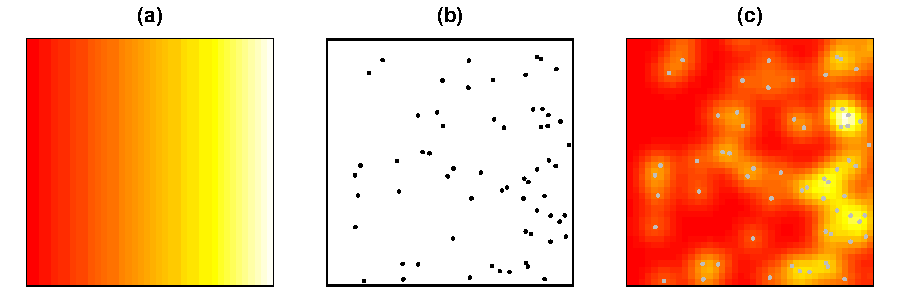
\includegraphics[width=\textwidth]{densities.pdf}
\caption{Examples of (a) an expected AC density surface, (b) a realisation of ACs from this density surface, and (c) the associated realised usage density surface (with ACs shown as grey dots).}
\label{fig:densities}
\end{figure}

\subsection{Estimated density surfaces}

If we are interested in explaining why density tends to be high in some places and lower in others, or in characterising the process that governs the distribution of ACs, then we are primarily interested in estimating a density surface like that shown in Figure~\ref{fig:densities}(a). In this example, it is easting that influences this density, but in general it might be any of a wide variety of habitat or environmental covariates, some of which may be unobserved and evidenced only by spatial clustering of ACs. 

If we are interested only in where the ACs are, and not in explaining why they are there, then Figure~\ref{fig:densities}(b) suffices. But suppose that we observe ACs with some error. For example, Figure~\ref{fig:acesterr} shows the distributions of estimated AC locations when the locations are estimated with bivariate normal errors with (a) small standard errors, (b) larger standard errors, and (c) standard errors increasing linearly from the centre of the plot. The estimation uncertainty ``spreads'' each AC according to a bivariate normal distribution, with greater spreading when there is greater uncertainty.

\begin{figure}[htbp]
\centering
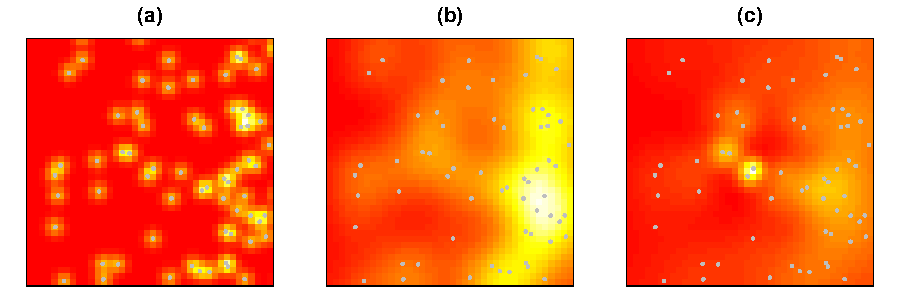
\includegraphics[width=\textwidth]{acesterr.pdf}
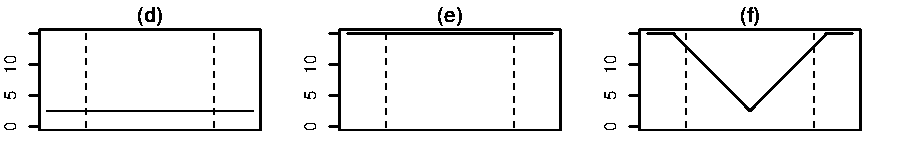
\includegraphics[width=\textwidth]{sigmas.pdf}
\caption{Examples of the density of the ACs of Figure~\ref{fig:densities}(b), when observed with bivariate normal estimation errors with standard errors (a) $\sigma=2.5$, (b) $\sigma=15$, and (c) $\sigma=2.5$ at the centre of the plot, rising linearly to $\sigma=2.5$ by the edge of the plot. True ACs shown as grey dots. The colour scales of panels (a) to (c) are such that the highest and lowest densities in each plot is the same.
Panels (d) to (f) plot the standard errors of the observation errors against the x-axis. Vertical dashed lines show the extent of the survey region in panels (a) to (c); a buffer beyond this is included because spreading of points outside it affect the plot within the survey region.}
\label{fig:acesterr}
\end{figure}

Ignoring the actual AC dots (because they cannot be observed), Figure~\ref{fig:acesterr}(a) gives a reasonable visual representation of where the ACs are. It is much more difficult to pick out individual ACs from Figure~\ref{fig:acesterr}(b), but it gives a reasonable representation of where the high- and low-density regions of ACs are -- much like Figure~\ref{fig:densities}(a), but customised somewhat for this particular realisation of AC locations rather than their long-run average locations. Note, however, that these two figures are representations of exactly the same set of ACs and that if one interprets them as plots of AC density, they contradict each other. Figure~\ref{fig:acesterr}(a) says that almost all the region has low density (red in the plot) and that there are lots of small high-density regions, while Figure~\ref{fig:acesterr}(b) says that there is much less variation in density, that there are large swathes of higher density (the yellow towards the right) and large swathes of low density towards the left. The reason that Figure~\ref{fig:acesterr}(b) shows less variation in density is not that there is less variation in the population (there are exactly the same ACs in both (a) and (b)), it is that we are less sure about the location of the ACs in (b). To interpret this as less variation in AC density is to invite incorrect ecological inferences.

Now what about Figure~\ref{fig:acesterr}(c)? If this is interpreted as indicating where the high and low-density regions are, it is misleading. It says that the highest density region is in the centre of the plot, and that the region with most variation in density is the central region, which is not true. 

The fact that there is only small observation error in the centre of the plot and large observation error at the edges means that the ACs near the centre are not spread much and therefore appear as higher peaks in the surface, with low regions where there are no ACs. Near the edges of the plot, on the other hand, observation error is high and ACs are spread a lot, which both flattens the peaks at individual AC locations and ``fills in'' the troughs where the are no ACs. We see the same effect with the usage density maps (Figure~\ref{fig:acuseesterr}), but less pronounced because the usage about the ACs already ``spreads'' around points before any observation error occurs.

\begin{figure}[htbp]
\centering
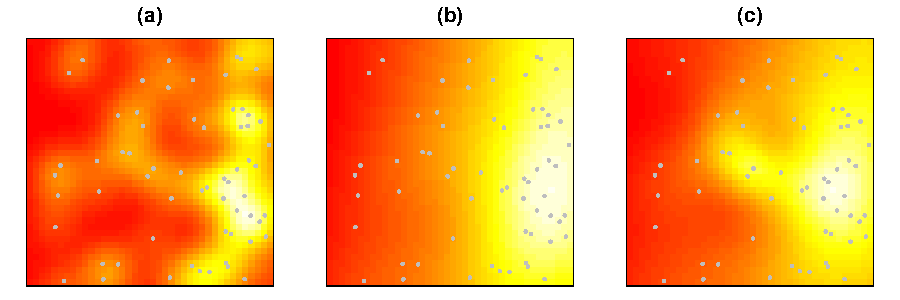
\includegraphics[width=\textwidth]{acuseesterr.pdf}
\caption{Examples of the usage density of Figure~\ref{fig:densities}(c), when observed with bivariate normal estimation errors with standard errors (a) $\sigma=2.5$, (b) $\sigma=15$, and (c) $\sigma=2.5$ at the centre of the plot, rising linearly to $\sigma=2.5$ by the edge of the plot. True ACs shown as grey dots. The colour scales of the three plots are such that the highest and lowest densities in each plot is the same.}
\label{fig:acuseesterr}
\end{figure}

It is a feature of SCR surveys that the locations of individuals farther from the detector array tend to be estimated with greater uncertainty than individuals within the array. This is illustrated in Figure~\ref{fig:screrr}, which shows the estimated probability density functions for two animals detected on a simulated SCR survey with a 4$\times$4 array placed in the centre of the population shown in Figure~\ref{fig:densities}(b). The reason contours top right ``avoid'' the triangle is because the detection function range, estimated from the whole survey, not just the points shown, is large and if the AC was near the triangle, other detectors would have high probability of detecting it. The fact that they did not makes them ``repel'' the AC. %\todo[inline,size=\footnotesize]{BCS: How come the contours in the top-right are avoiding the black triangle? Shouldn't the contours be happy to cover the triangle, because the animal was detected there?\\ DLB: This is because the detection function range (estimated from the whole survey, not just the points shown) is large and if the AC was near the triangle, other detectors would have high probability of detecting it. The fact that they did not makes them ``repel'' the AC. I've added this to the text.}

\begin{figure}[htbp]
\centering
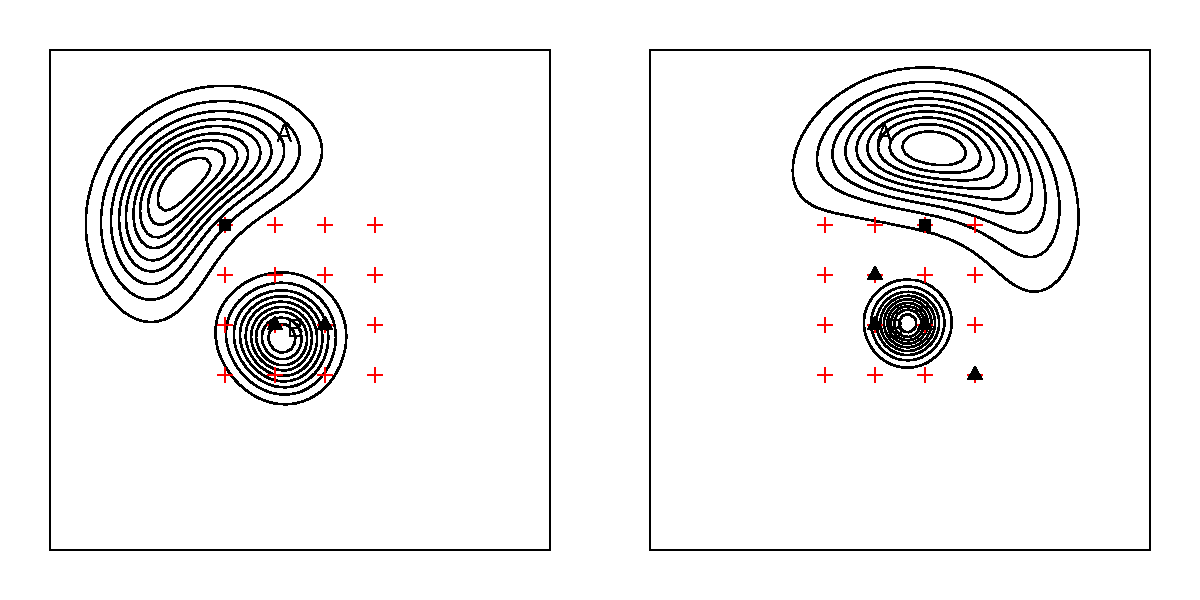
\includegraphics[width=0.5\textwidth]{screrr.pdf}
\caption{Estimated probability density function contours for two detections in an SCR survey of the population shown in Figure~\ref{fig:densities}(b). Detectors are shown as red crosses. The lower left individual was detected at detectors indicated by black squares, the upper right individual only by the top right detector indicated by a black triangle.}
\label{fig:screrr}
\end{figure}

%FROM BEN: Give examples of papers where people have misinterpreted the sum of posterior AC distributions under either definition (1) or (3) above. Dorazio uses interpretation (1) because they explicitly talk about the distribution of ACs. Alexander et al. is a little ambiguous, and could be either definition (1) or (3) depending on whether or not they are talking about density under their particular realisation of the state process, but not (2), because they refer to "density of animals" and not "ACs". Elliot \& Gopalaswamy (2017) do the same thing as Alexander et al. in their caption of Fig 2.

%As a motivating example for the categorisation above, suppose that animals' activity centers have been generated by a point process whose intensity surface is shown in Figure \ref{introplot}a (with intensity increasing eastwards), and with a single realisation of this process overlain (as black dots). In reality the locations of the dots are unknown and must be estimated, but whether the estimated locations of the dots are of interest themselves, or only as a means of estimating the underlying intensity surface, depends on what the goal of the analysis is. If one is interested in where activity centers currently are, one is looking for the dots. If one is interested in which areas are favourable for the location of activity centers {\it in general}, then the dots are only a means with which to estimate the underlying intensity surface. The interpretation of these surfaces differs, but so does their estimation. 

%Expected activity center densities are estimated by modelling the intensity of the state process as a function of environmental covariates, realised activity center densities by summing posterior activity center densities across detected and undetected animals.

%Figure \ref{introplot}b imagines that these realised locations were observed with some small amount of measurement error, and plots the sum of the ``posterior distributions'' for each point that account for this uncertainty. This is -- ignoring for now the complexities of fitting an SCR model -- the surface that we argue is incorrectly interpreted as a species distribution model. It is clearly different to the underlying surface shown in Figure \ref{introplot}a. Figure \ref{introplot}c introduces animal movement around the ACs, representing the expected density of animals at locations at an arbitrary discrete point in time. The estimation of realised animal densities has not been previously described, but also sums posterior densities across animals (we describe this in more detail in Section ???). The surfaces in Figure \ref{introplot}a-c represent the three kinds of animal density surfaces described above -- expected activity center density, realised activity center density, and realised animal density, respectively. A key point we return to in several places in the paper is that these three surfaces are all of potential ecological interest, but that they differ in fundamental ways, and that it is important to keep the distinctions between the surfaces clear.

%\begin{figure}[htbp]
%\centering
%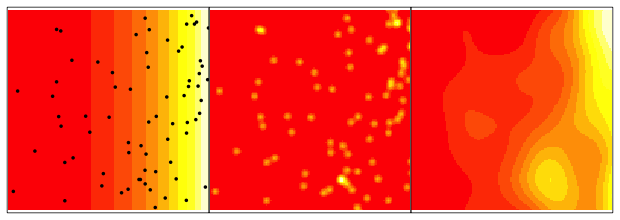
\includegraphics[width=\textwidth]{density-plots.png}
%\caption{Simulated activity centers (black dots, left-hand panel) generated from a point process with intensity increasing from left to right (surface in left-hand panel), estimates of those activity centers (central panel), and estimates of animal locations (right-hand panel). These represent, respectively, what we term expected activity center, realised activity center, and realised animal density surfaces.}
%\label{introplot}
%\end{figure}

%The remainder of the paper illustrates the dependency of the realised activity center density on detector location using three example datasets of increasing complexity. The first (Section \ref{1dbinom}) simulates a fixed number of animals from a one-dimensional binomial point process, assumes that animals do not move and also assumes an extremely simple detection process. This example primarily illustrates that flat density surfaces away from detectors reflect a lack of knowledge of the locations of unobserved animals, and not that the realised activity center density is constant.

%The second example (Section \ref{monalisa}) simulates a more realistic two-dimensional Poisson point process. For visual impact our simulated data is drawn from a density surface model based on one of the most recognisable images in Western culture, the Mona Lisa. This example demonstrates that the realised activity center density is dependent on where detectors are located, both far from the detectors and, perhaps less obviously, in and around the detectors. It also introduces the use of covariates as a means of estimating expected activity center densities, and also incorporates animal movement into realised animal density maps.  

%A third and final example (Section \ref{nagarahole}) reanalyses data from a previously published study using SCR to estimate the realised activity center density of tigers in the Nagarahole Tiger Sanctuary \cite{?}. This survey used a dense network of detectors; by removing some of these we show the dependency of the density surface on detector locations using real data. A discussion section (Section \ref{discussion}) summarizes our main points, and a final section concludes.



%\section{Simulating a 1-D binomial point process} \label{1dbinom}

%\subsection{Materials and methods}
%We simulate a fixed number of animals distributed across a single dimension according to a linear trend, and then model this data using a binomial point process that incorrectly assumes a uniform distribution of animals across space. Here one can think of, for example, a situation in which true density strongly depends on a covariate that varies in space, but that this covariate is unknown. 

%We place a fixed number of points $N$ at random locations on the interval $0<x<R$, with $R=15$. Points are generated according to a probability density that makes them more likely to appear near $x=0$ than $x=15$ i.e.\ $f(x)\propto 1-x/15$ for $0<x<15$ and $f(x)=0$ otherwise.

%For simplicity we divide the interval into $R=15$ equal-sized regions, thinking of these as cells in a one-dimensional grid. detectors are placed in $T=5$ cells. We make the simplifying assumptions that animals do not move from the cell they are placed in, and that each detector detects animals perfectly within the cell it occupies but cannot detect animals beyond that cell. 

%We simulate with $N=50000$ animals and with different detector configurations.

%\subsection{Results}
%Figure \ref{binom} shows the estimated realised activity center densities -- the estimated number of activity centers for $N=50000$ animals distributed according a binomial point process with density decreasing linearly with $x$. Under the extremely simplified conditions of this example (no movement of animals, perfect detection within cells), SCR recovers the true number of activity centers in each cell that contained a detector, knows how many animals were {\it not} detected\footnote{Here this is because $N$ is known but if $N$ is unknown it can be estimated. A model assuming a constant density and detecting $n$ animals from a perfect survey of $T/R$ of the study area estimates the total number of animals to be $\hat{N}=n/(T/R)$, implying there are $\hat{N}-n$ animals in the area that were not detected by any detector.}, and distributes the activity centers of these undetected animals evenly across the cells that do not contain a detector\footnote{$\hat{N}-n$ activity centers distributed uniformly between $R-T$ detectorless cells gives a mean of $(N-n)/(R-T)$ activity centers per cell, close to the mean of the underlying process $N/R$ when $n\ll N$ and $T\ll R$, as would usually be for wildlife surveys.}. 

%\begin{figure}[htbp]
%\centering
%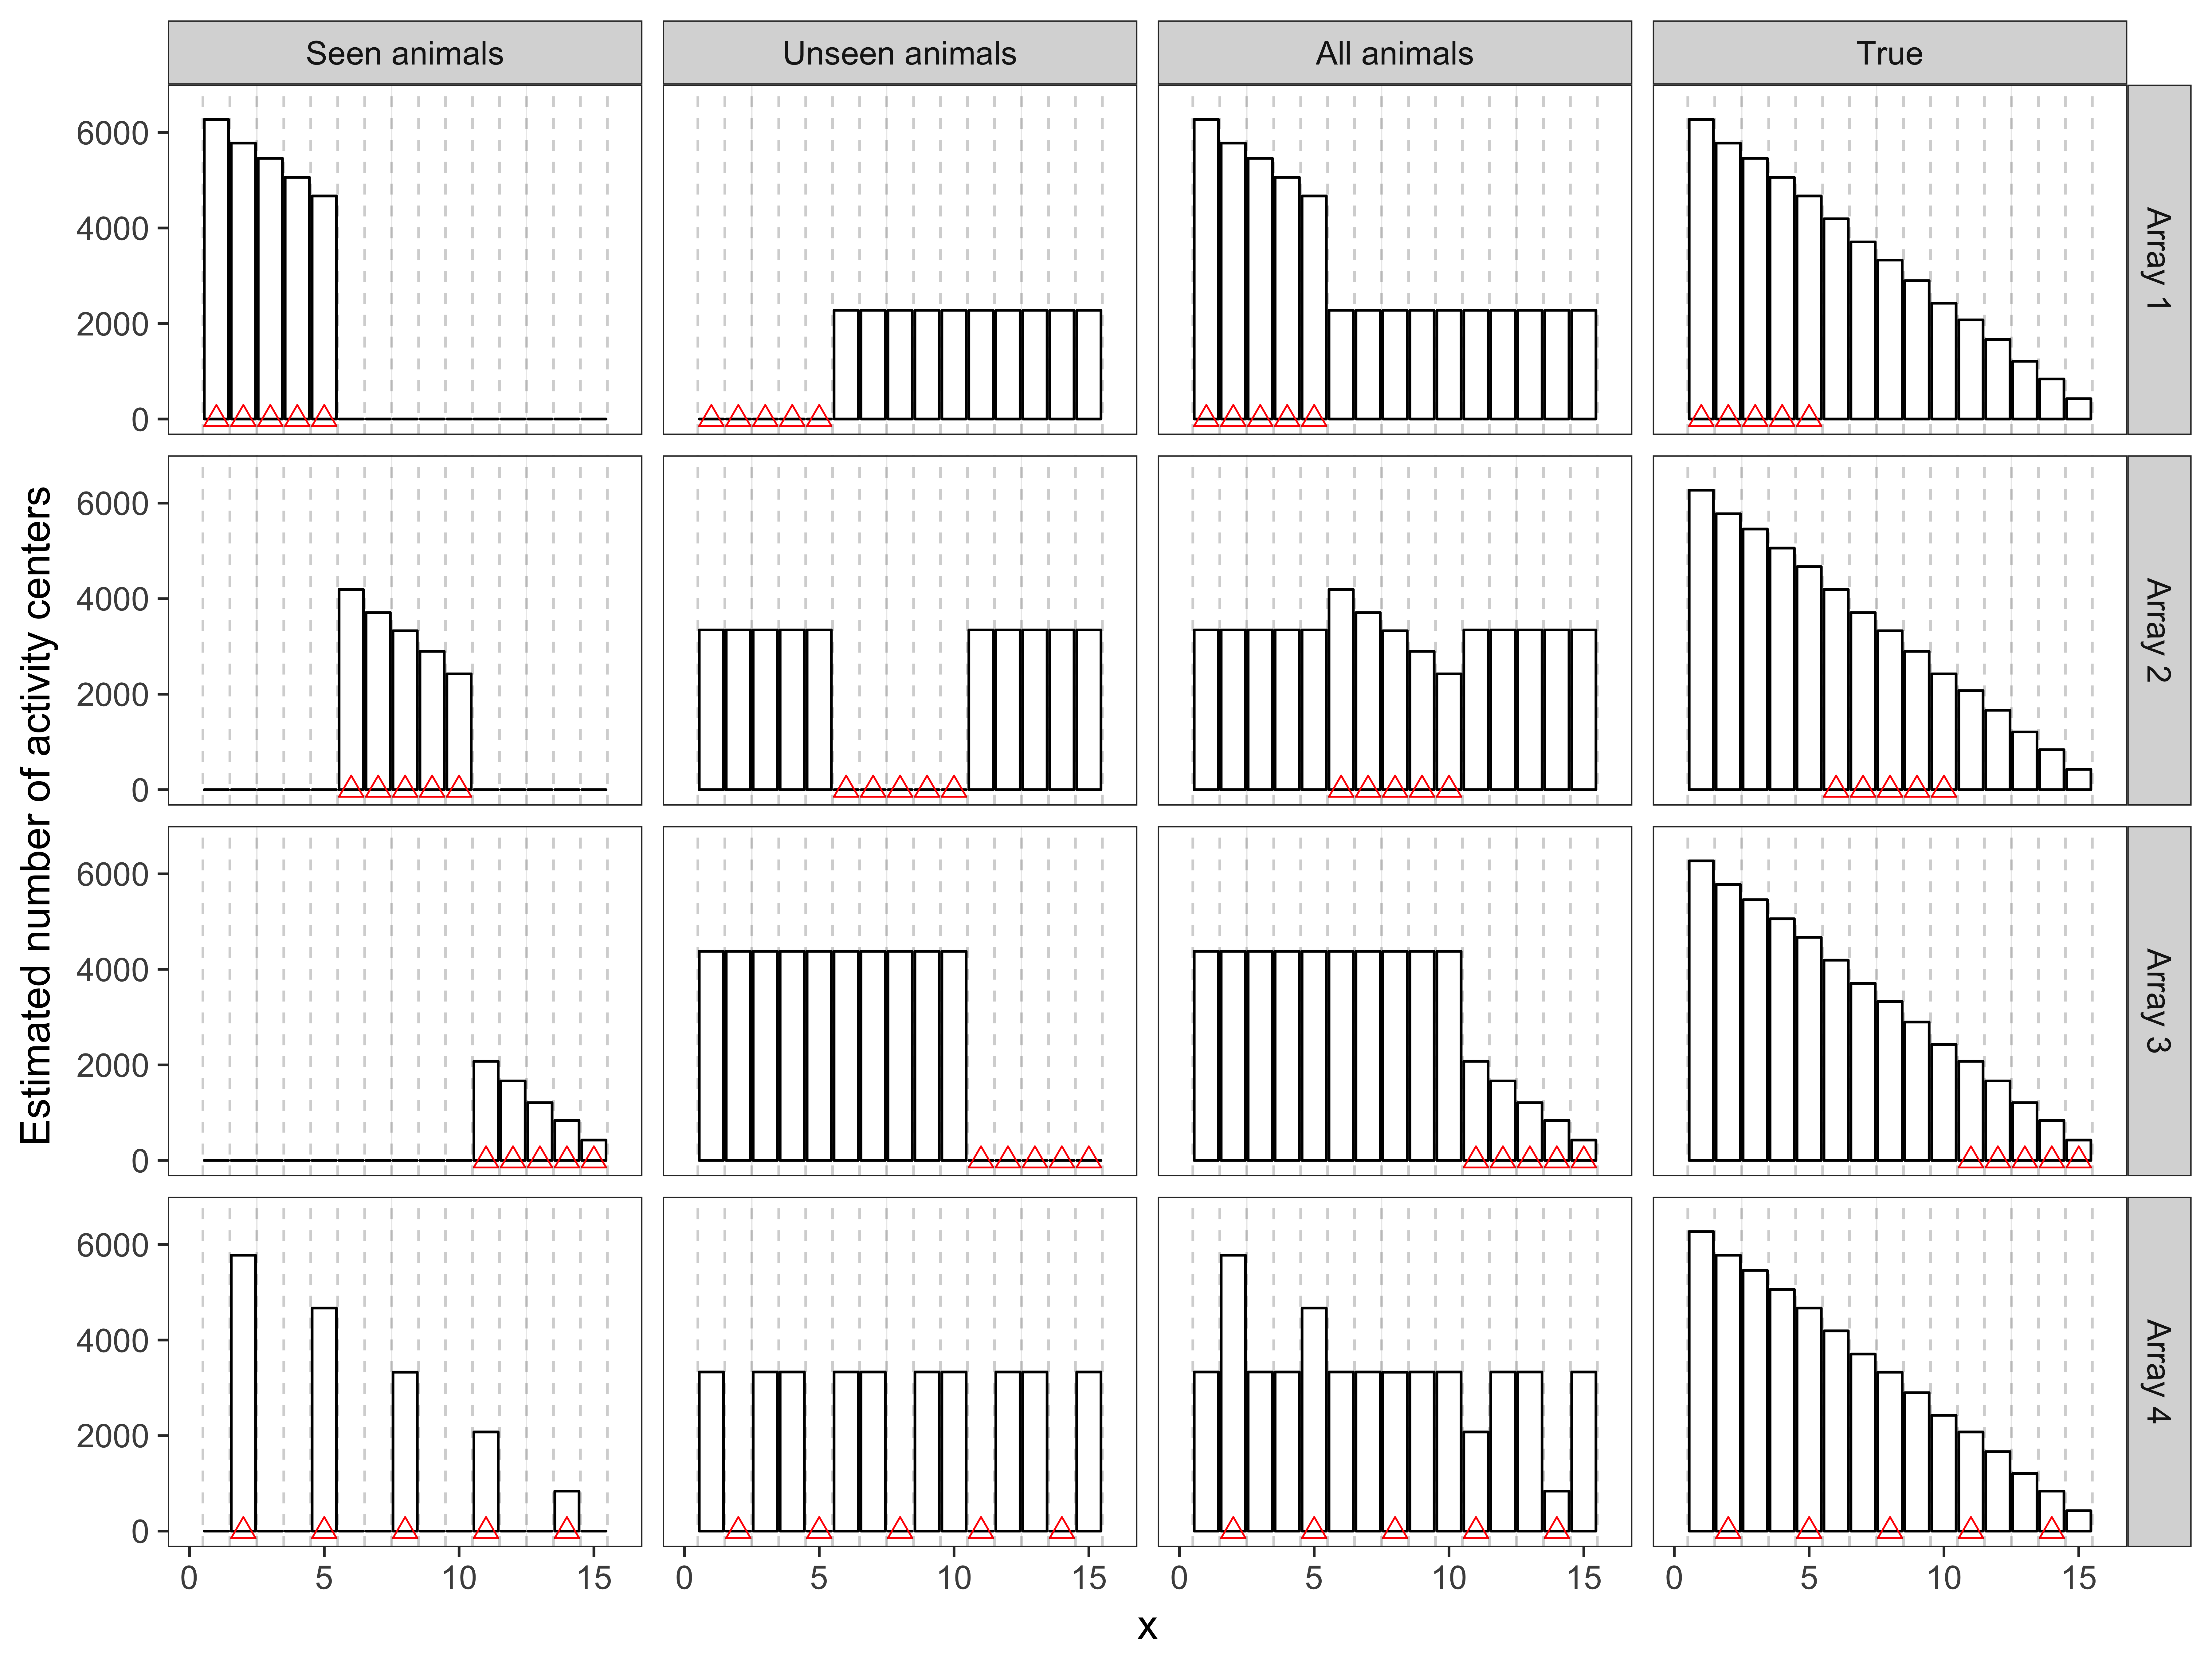
\includegraphics[width=1\textwidth]{binompp_inf.png}
%\caption{Estimated numbers of activity centers obtained from a binomial point process with $N=50000$ simulated animals and density decreasing linearly with $x$, no animal movement, and a step detection function that is perfect within cells and zero otherwise.}
%\label{binom}
%\end{figure}

\section{SCR density estimation methods} \label{secrmethods}

Maximum likelihood (ML) and Bayesian SCR estimation methods are documented in a good number of papers, starting with \cite{Borchers+Efford:08} and \cite{Royle+Young:08}, and we do not repeat the details here. Both ML and Bayesian inference are based on SCR likelihood functions that include a component specifying the AC density surface, which may depend on spatially-referenced covariates (the linear density surface shown in Figure~\ref{fig:densities}(a) is an example). The density surface is typically of the form $D(\bm{s})=\exp\left\{\beta_0 + \sum_{k=1}^K\beta_kx_k(\bm{s})\right\}$, where $\bm{s}$ is a point in the plane, $x_k(\bm{s})$ is the $k$th of $K$ spatially-referenced covariates, evaluated at $\bm{s}$, $\beta_0$ is and intercept parameter, and $\beta_k$ is the slope parameter for the $k$th spatially-referenced covariate. ML and Bayesian methods are able to estimate $\beta_0,\ldots,\beta_K$, and hence to estimate the expected AC density surface. 

Given spatial capture histories, ML and Bayesian methods are also able to estimate the locations of ACs (like those shown in Figure~\ref{fig:densities}(b), for example). While ACs are points, there is always uncertainty associated with estimating their locations, so that SCR estimates of AC locations are probability density functions (PDFs), not points. Estimates of these PDFs are conditional on the spatial capture histories of the individuals concerned -- because the capture histories contain the information on where each animal's AC was (see the capture histories and estimated location densities in Figure~\ref{fig:screrr}, for example). Details of how one obtains these estimated AC PDFs are contained in Section 4.3 of \cite{Borchers+Efford:08} for ML methods and the section ``Estimating derived parameters'' on page 3238 of \cite{Royle+al:09b} for Bayesian methods.

Note that we can obtain AC PDFs for undetected animals, because although the animals were unobserved, we know their capture histories -- namely no capture at every detector. Note also that all undetected animals will have the same AC PDF\footnote{This is not the case if there are individual-level covariates that affect detection probability estimates, but this is a complication that we ignore here in order to present as clear and uncomplicated an exposition of they key points of this paper as we can.} because they all have the same capture history. 

Suppose that we estimate from an SCR survey that there are $\hat{N}$ animals within the survey region. If one adds up the AC PDFs for all $n$ detected animals, and the $\hat{N}-n$ AC PDFs of the undetected animals, at all points in the survey region, one gets a surface that is in many publications (including those listed in the Introduction) interpreted as a density surface for ACs, or sometimes for animal locations. This is an estimate of the realised AC density.

It has been referred to as the estimated distribution, or density of \textit{animals}. However, animals distribute themselves around their ACs, so that AC density and animal density are not the same thing. Suppose for example, that we are certain that there is exactly one AC in a region that has surface area 1 (so that AC density in this region is 1). Suppose also that the animal with AC in this region ranges wider than this region, and spends exactly half its time in this region. It is not certain that there is an animal in the region at any time, so that animal density will be less than 1. In this example, it would be fair to say that the \textit{animal} density in the region is 0.5. To avoid confusion, we refer to this as the ``usage density'' rather than ``animal density''. Details of how one estimates the realised usage density surface from an estimate of the realised AC density surface are given in Appendix~\ref{appx:usage-details}.

In summary, there are three kinds of estimated surface of interest here: 
\begin{itemize}
\item An estimate of the expected AC density surface: This is an estimate of the density model component of the SCR model, which governs the number and locations of ACs.
\item An estimate of the realised AC density surface: This is the combined estimates of realised AC densities of all animals, conditional on each animal's capture history.
\item An estimate of the realised usage density surface:  This is the combined space usage density of animals, conditional on each animal's capture history.
\end{itemize}

\section{Methods}

We illustrate what each of the three kinds of estimated surface gives the practitioner, and what interpretations of the surfaces are valid and useful, by (a) simulating data from a density surface that has easy visual interpretation, and (b) using the Nagarahole SCR tiger survey data kindly provided by the first author of \cite{Dorazio+Karanth:17}.

\subsection{Reproducing the Mona Lisa} \label{monalisa}

For easy visual interpretation, we turned one of the most recognisable images in Western culture, the Mona Lisa, into a density surface. We created a $50 \times 50$ pixel greyscale version of a region of the original image (Figure \ref{mlinputs}, ``True Density'') in which greyscale values give the true density of ACs, and lighter areas correspond to higher densities.

We then rescaled the image's pixel intensities to generate two density surfaces. In one of these, pixel intensities were rescaled so that their sum (corresponding to the expected number of activity centers over the surface) was 7,500. In the other, pixel intensities were rescaled so that their sum was 80. We then used each density surface to generate a realisation of points from the underlying process. A single draw from the first surface (a Poisson distribution with mean 7,500) resulted in 7,451 ACs being generated, which we plot in Figure \ref{mlinputs}, ``Realisation 1''. This realisation has the advantage of closely reproducing the source image, and when we conduct SCR surveys with this population, it gives us an indication of the asymptotic behaviour of SCR density estimators, i.e. as sample size gets very large. A draw from the second surface (a Poisson distribution with mean 80) produced a much smaller realisation of 84 points (Figure \ref{mlinputs}, ``Realisation 2''). This realisation captures the Mona Lisa only at an extremely gross level (the darkest region corresponding to the hair can be picked out if you squint at the image long enough!), but is a useful aid to understanding some properties of the estimators.

%We then used the density surface to generate two realisations of points from the underlying process. In the first of these we generated the number of points from a single draw from a Poisson distribution with mean 7,500, resulting in 7,451 ACs being generated, which we plot in Figure \ref{mlinputs}, ``Realisation 1'' as a density at $50\times 50$ pixel resolution. This realisation has the advantage of closely reproducing the source image, and when we conduct SCR surveys with this population, it gives us an indication of the asymptotic behaviour of SCR density estimators, i.e. as sample size gets very large. We also generated a much smaller second realisation of 84 points (Figure \ref{mlinputs}, ``Realisation 2''). This realisation captures the Mona Lisa only at an extremely gross level (the darkest region corresponding to the hair can be picked out if you squint at the image long enough!), but is a useful aid to understanding some properties of the estimators.

\begin{figure}[htbp]
\centering
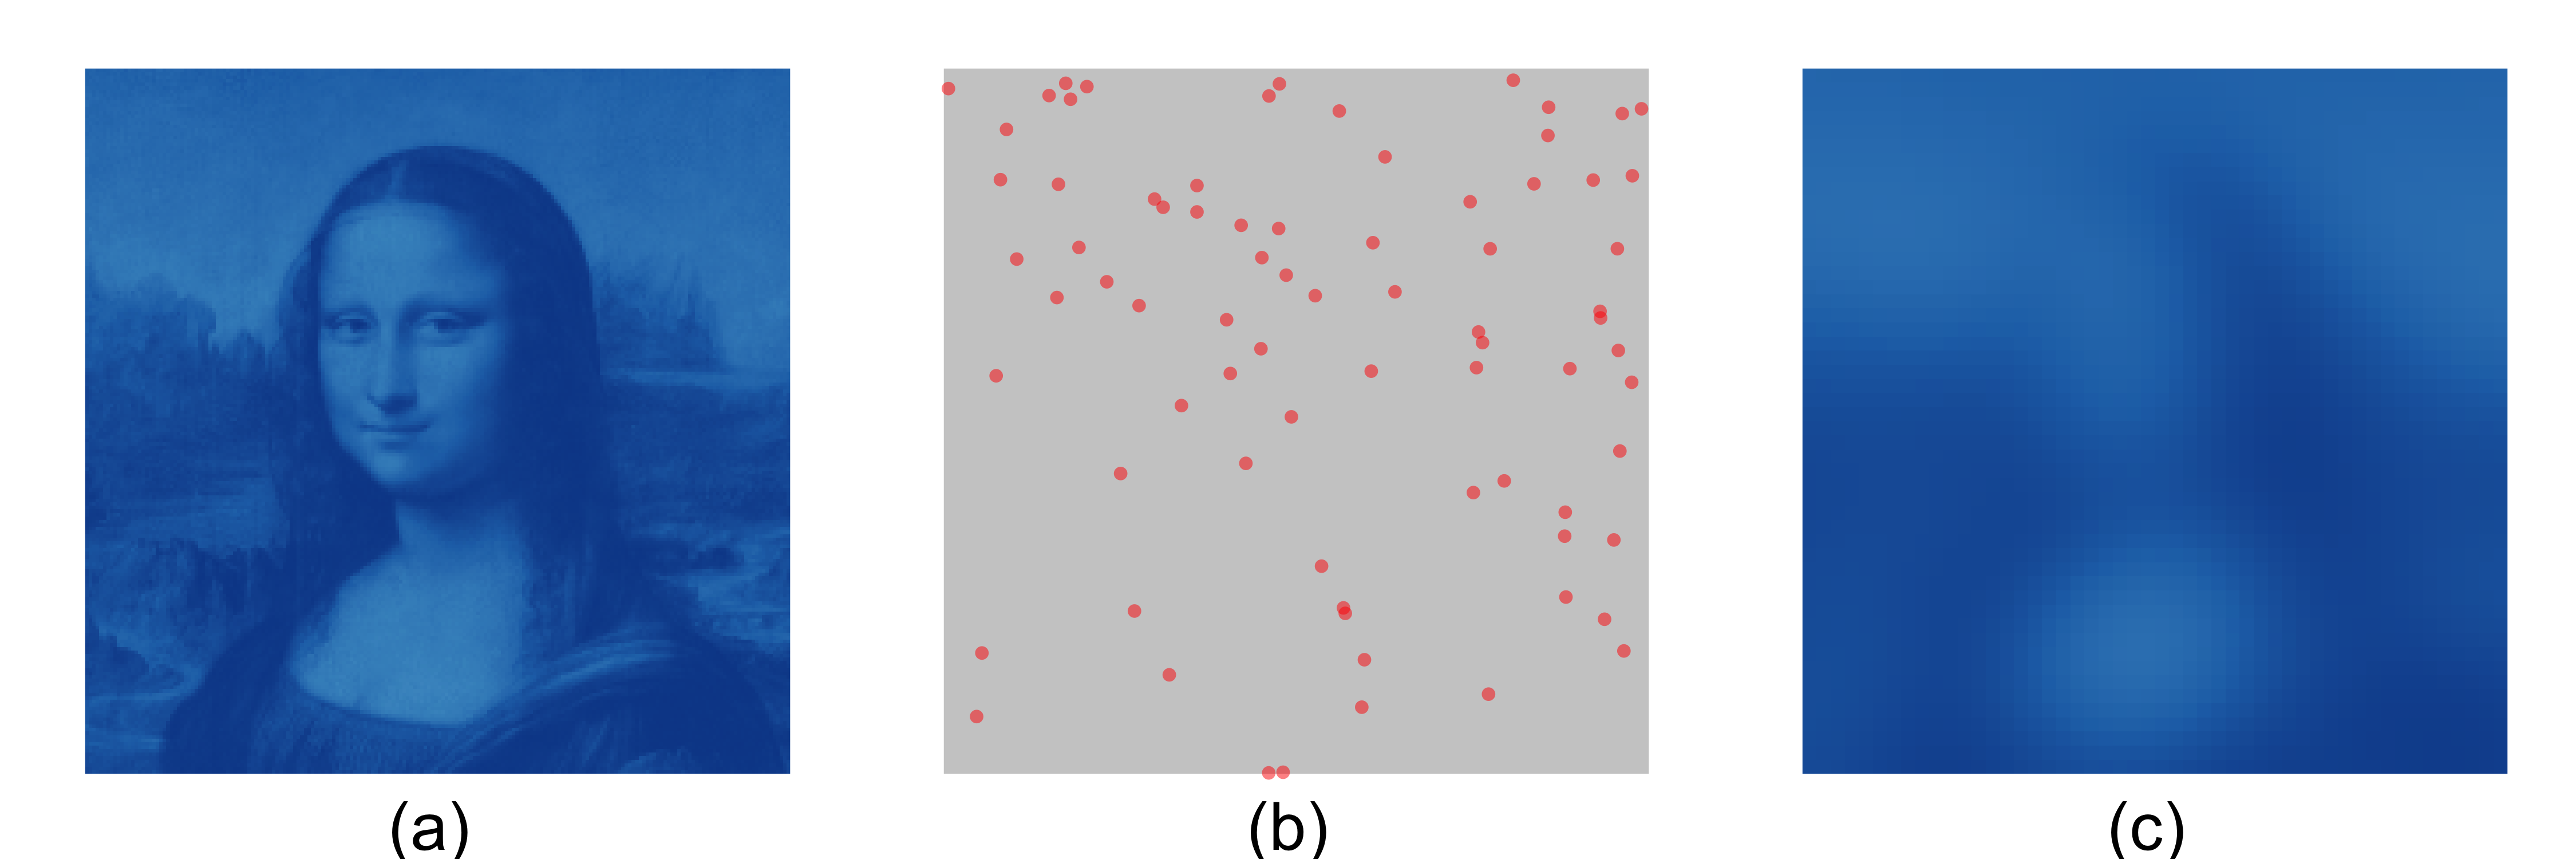
\includegraphics[width=1\textwidth]{mona_inputdata.png}
\caption{Input data for the Mona Lisa simulation study. A greyscale version of the Mona Lisa (``True Density'') is treated as an expected AC density surface, from which we generated a sample of 7,451 and 84 ACs and plotted these as realised AC density surfaces at $50\times 50$ pixel resolution (``Realisation 1'' and ``Realisation 2'', respectively).}
\label{mlinputs}
\end{figure}

We simulated SCR surveys of the population, using a variety of detector arrays and also varying sample size. Different arrays and detection functions were used for the large and small populations described above. With the large number of activity centers (``Realisation 1'' in Figure~\ref{mlinputs}), we used a $4\times 3$ array placed at four different locations (Figure~\ref{mona_torch_higheffort}). These have an average spacing of $2\sigma$ between detectors. We simulated capture histories using a half-normal encounter rate function with the spatial scale parameter $\sigma=2$. Simulated capture histories were Poisson random variables with expected values equal to the encounter rate function evaluated at the distances of detectors from ACs. In order to investigate the asymptotic behaviour of the realised and expected AC density surfaces we simulated very large samples from each array by using a baseline encounter rate hazard of $\lambda_0=13.8$, which gave an average of 1,150 detected animals and 11,304 detections (i.e.\ an average of about 10 detections per animal) over 100 simulated capture histories (always using the same animal population). 

When using relatively few activity centers (``Realisation 2'' in Figure~\ref{mlinputs}), visual interpretation was made easier by increasing the spatial scale parameter, effectively increasing the distance animals travel from the activity centers, and also by increasing the distance between detectors. For these cases, we increased $\sigma$ to 4, holding other detection function parameters at their previous values, and used a $3 \times 3$ array with an average spacing of $2\sigma=8$ between detectors, double that used previously. We used two different locations of the detector array and simulated capture histories with three different survey effort levels, obtained by varying $\lambda_0$ between 2.07 and 6.9 and generating between 79 and 526 detections of between 31 and 44 individuals (see Figure~\ref{mona_peaky_avgd}). After simulating capture histories for these arrays, we estimated the realised and expected AC surfaces for each simulation. 

To estimate the realised AC surface, we assumed a model with constant density. To estimate an expected density surface, we generated covariates by manipulating the true density surfaces to blur them, using two levels of blurring, as shown in Figure~\ref{mona_peaky_avgd}, with either a strong (relatively little blurring) or weaker (more blurring) covariate effect. Pixel intensities were rescaled after blurring so that the number of expected activity centers remained the same as in the original surface (i.e., either 7,500 or 80). Because they are based on true density, these covariates are very informative about the true densities although the strength of the association between the covariate and true density is substantially lower for the ``Moderate'' covariate. For each of these covariates we estimated a corresponding expected AC density. Note that, because density is parameterised with a log link (see Section \ref{secrmethods}) but the blurred surfaces were obtained directly from the true density surface (so that $D(\mathbf{s}\approx x_k(\mathbf{s}$, with the degree of blurring determining the accuracy of approximation), covariates needed to be log-transformed to ensure the model was correctly specified.

For each activity centre scenario, we simulated 100 capture histories (at each array, keeping the locations of activity centres fixed) and estimated the expected AC density surface, realised AC density surface and realised usage density surface for each simulated capture history. This allows us to average the density surfaces over repeated simulated surveys (for example, to show that differences between these surfaces the true population density surface are not a result of only a single survey being possible) as well as use the density surfaces from a single simulated survey (to show the typical output a researcher would obtain). We show both averaged and single-survey surfaces depending on our goals, making it clear in each case what we are referring to.\todo{Check wording of this. Need to check its clear which results are averaged} We used maximum likelihood inference using the {\it secr} package in R version 4.1.2 and Bayesian inference using the NIMBLE package, also in R.\todo{Is this right - NIMBLE?} Here were report on the maximum likelihood estimates; the Bayesian estimates are not materially different and are reported in Appendix~\ref{appx:Bayesinference}.\todo{Need to create the appendix.}

%We simulated capture histories and from them estimated the realised AC density surface and the realised usage density surface for each simulation and compared them to the true population density surface. We conducted maximum likelihood inference using the {\it secr} package in R version 3.4.3 and Bayesian inference using the NIMBLE package, also in R.\todo{Is this right - NIMBLE?} Here were report on the maximum likelihood estimates; the Bayesian estimates are not materially different and are reported in Appendix~\ref{appx:Bayesinference}.\todo{Need to create the appendix.}

\subsection{Results}

\subsubsection{Realised AC densities with many activity centers}

%The same patterns hold in two dimensions under the standard wildlife survey assumptions of Poisson-distributed activity centers (with constant intensity) and detectability inversely related to distance from activity center (Figure \ref{mona1low} and \ref{mona1hi}). A single sampling occasion was sufficient to capture the broad features of the Mona Lisa, but only close to where detectors were located (Figure \ref{mona1low}, first row). 

A striking feature of realised AC density surface estimates shown in Figure~\ref{mona_torch_higheffort} is that no matter where the array is placed, the region away from the array has a flat estimated density (which approaches the mean estimated density). Within the array, the realised AC surface estimate does a reasonable job of picking out the features of the Mona Lisa, but if we look at the region common to all arrays (within the dashed rectangle) we see that the realised AC surface estimate of this region is quite different for the four arrays. Estimates of the realised AC surface depend very strongly on where an array is placed -- recall that in these simulations the true ACs are in exactly the same place for all surveys and so none of the difference is attributable to ACs being in different places.

%Very different relative and absolute densities were obtained depending on where detectors are located, even when estimating density {\it in exactly the same region of the surface and where that region is close to the array} (Figure \ref{mona1low} and \ref{mona1hi}, second row). With a single occasion, density was always estimated to be highest nearest the corner where the detector is located (Figure \ref{mona1low}, second row). This pattern occured because the inset region happened to occur in a region of above average density. If instead it occured in a low density region one would see the opposite pattern -- low density in the corner containing a detector, increasing away from the detector. This was clearly visible when a single sampling occasion was used, because the estimated surface reverted quickly to the mean intensity. Additional sampling allowed fine detail in the density surface to be estimated close to detectors, with slower reversion to mean intensity, but there was still very clear disagreement between the density surfaces returned by the different arrays (Figure \ref{mona1hi}, second row).

\begin{figure}[htbp]
\centering
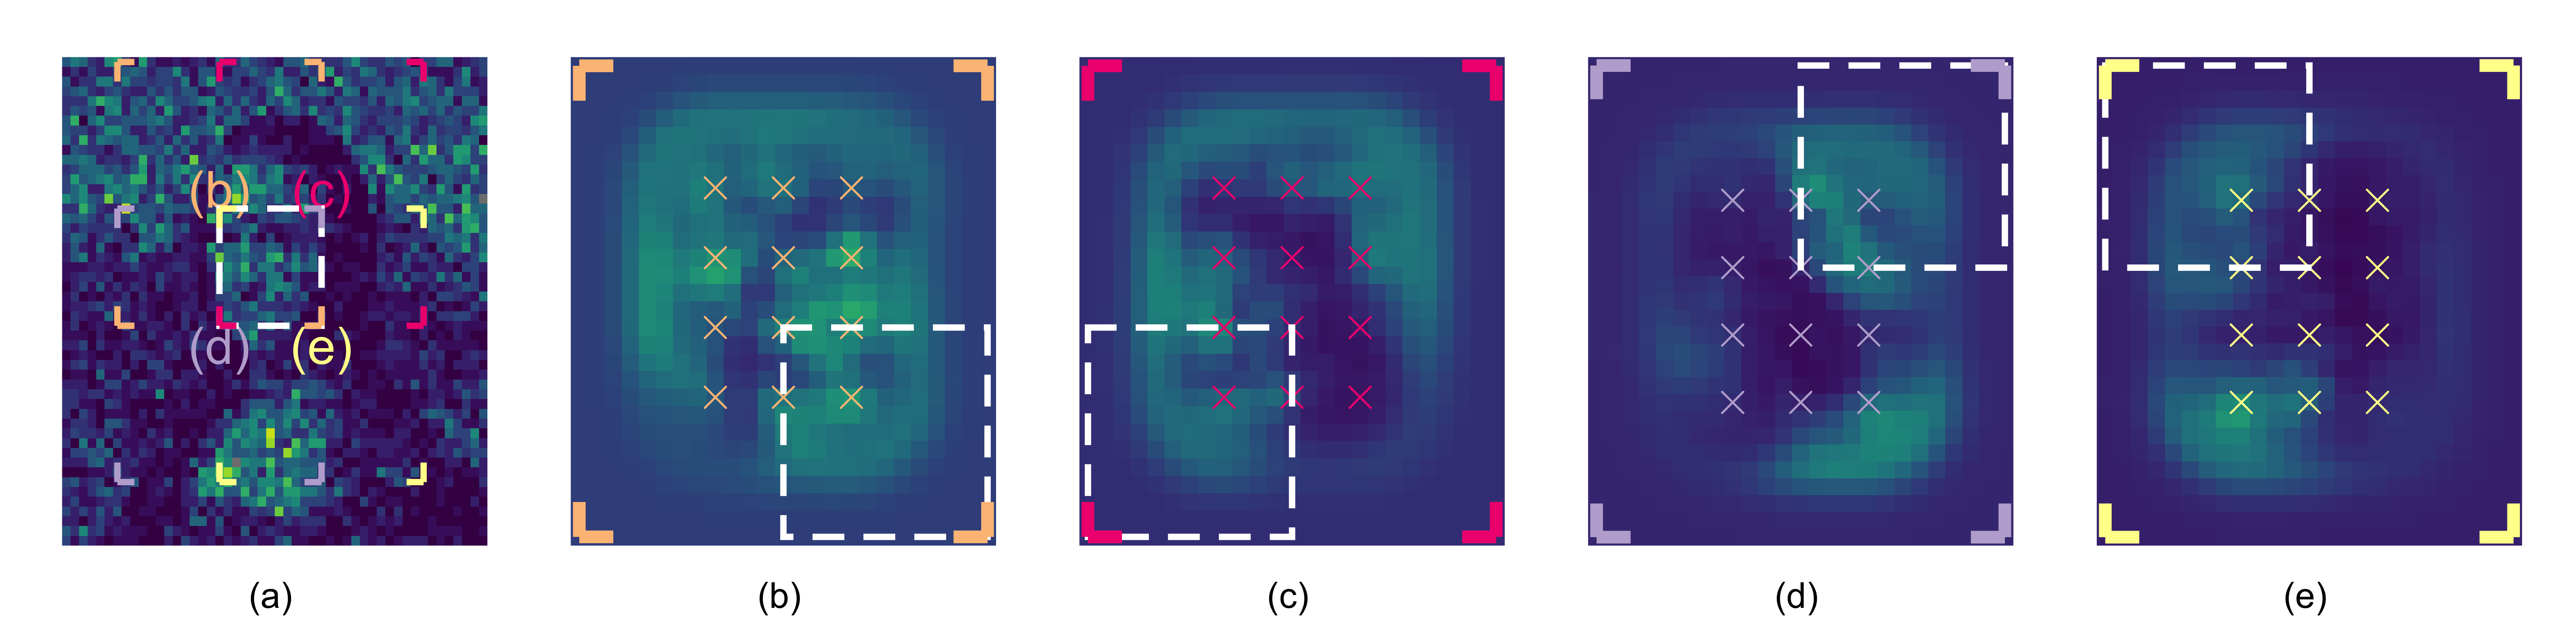
\includegraphics[width=1\textwidth]{mona_torch_higheffort.png}
\caption{Plot (a) shows the true AC densities. Plots (b), (c), (d) (e) show the estimated realised AC surfaces (averaged over 100 simulations) estimated using a 4$\times$3 array placed at four different locations. The orange, red, grey and yellow corner marks in plots (b) to (e) indicate the location of each of (b) to (e) in plot (a). The white dashed box located in the centre of the Mona Lisa's face in plot (a) is also shown in plots (b) to (d) so that one can easily compare the predictions of the centre of the face from each array.}
\label{mona_torch_higheffort}
\end{figure}

%\todo[inline,size=\footnotesize]{The densities in these plots should really be expected densities (i.e. averages over lots of simulations) - particularly for the bottom row of estimates, since you might expect substantial random variation in these from sample to sample. The top images illustrate fairly convincingly how the SCR ``torch'' does pretty well where it ``shines'' but can't see beyond, without the need to use expected values, but because you can't see pattern in the bottom ones, you are more inclined to say ``So what that they are not the same - there is sampling variation.'' Also, we need to give sample sizes for these surveys (number detections and number of different individuals).}

%\begin{figure}[htbp]
%\centering
%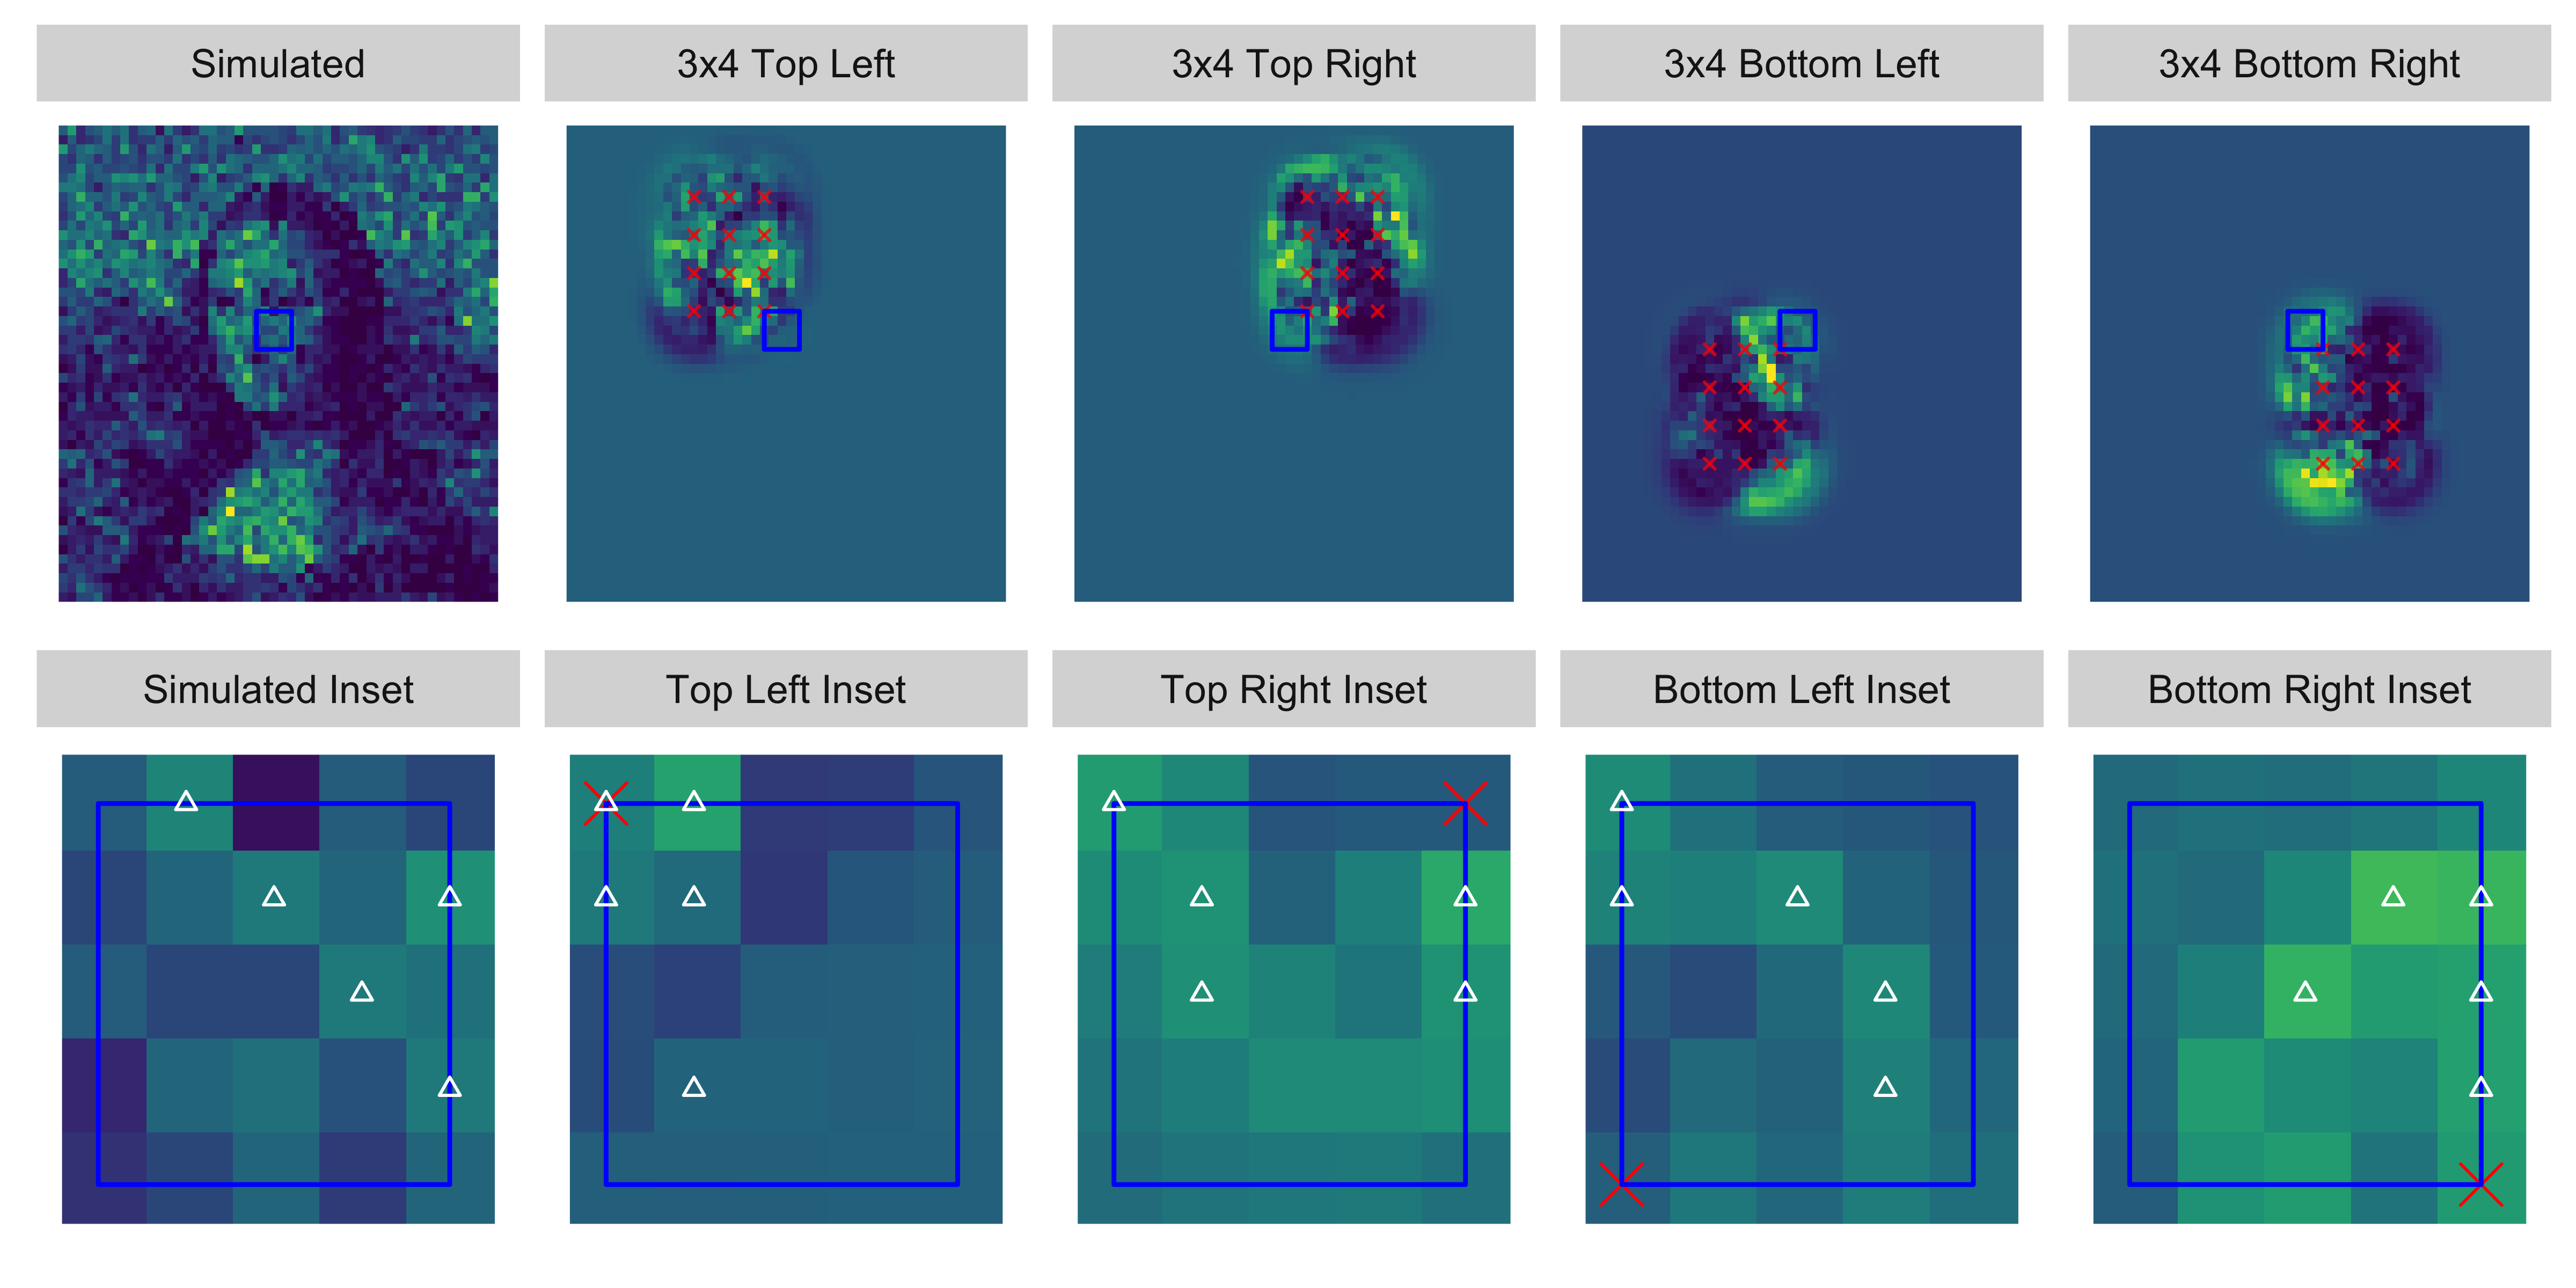
\includegraphics[width=1\textwidth]{many_faces_mona_higheffort.png}
%\caption{Need to replace this figure. %True activity center densities in this realisation (``Simulated'') compared with activity center surfaces estimated using different arrays after 20 sampling occasions. High density areas are indicated in yellow, low density areas in blue. See the caption to Figure \ref{mona1low} for further annotation details.
%}
%\label{mona1hi}
%\end{figure}

\subsubsection{Expected activity center densities with many activity centers}

Introducing covariates into the density models allowed us to recover features of the Mona Lisa across the entire image, not just near where detectors were located (Figure~\ref{mona_covariates}). Recovery will seldom be this good in reality - we have covariates that are more strongly related to true density than would usually be obtainable. Notwithstanding this, it is true in general that because the expected AC surface depends on the relationship between the covariate and density, the model uses estimates of this relationship obtained where it has lots of information (within the array) to infer density beyond the array. From a single survey\footnote{With such large sample sizes estimates of model coefficients show almost no variability from survey to survey and hence the expected AC surface, which is based on these coefficients, is also nearly identical between surveys. It makes almost no difference whether the results are averaged over repeated simulated surveys or not: the resulting expected AC surfaces are almost identical.}, with our ``Strong'' covariate (Figure~\ref{mona_covariates}a-c) we recovered all of the broad features of the Mona Lisa, and many of the fine scale features such as eyes, shading of clouds, {\it etc}. With the ``Moderate'' covariate (Figure~\ref{mona_covariates}d-f) we recovered broad scale features but no finer details. Importantly, the estimates within the dashed rectangle are almost identical for all array placements - these estimates are not sensitive to where the array is placed.

%With a ``weak'' covariate, the estimated density surface essentially reverted to the mean intensity of the process across the entire region. With a ``locally strong'' covariate -- one that is a good indicator of density in some parts of the study region but poor elsewhere -- the dependency on array location was reintroduced. If the array was located where the covariate was strong, the estimated density surface was accurate in that vicinity. If the array was located where the covariate was weak, then the model estimated no relationship between covariate and density and reverted back to the mean intensity everywhere in the region (Figure \ref{covariates}). 

\begin{figure}[htbp]
\centering
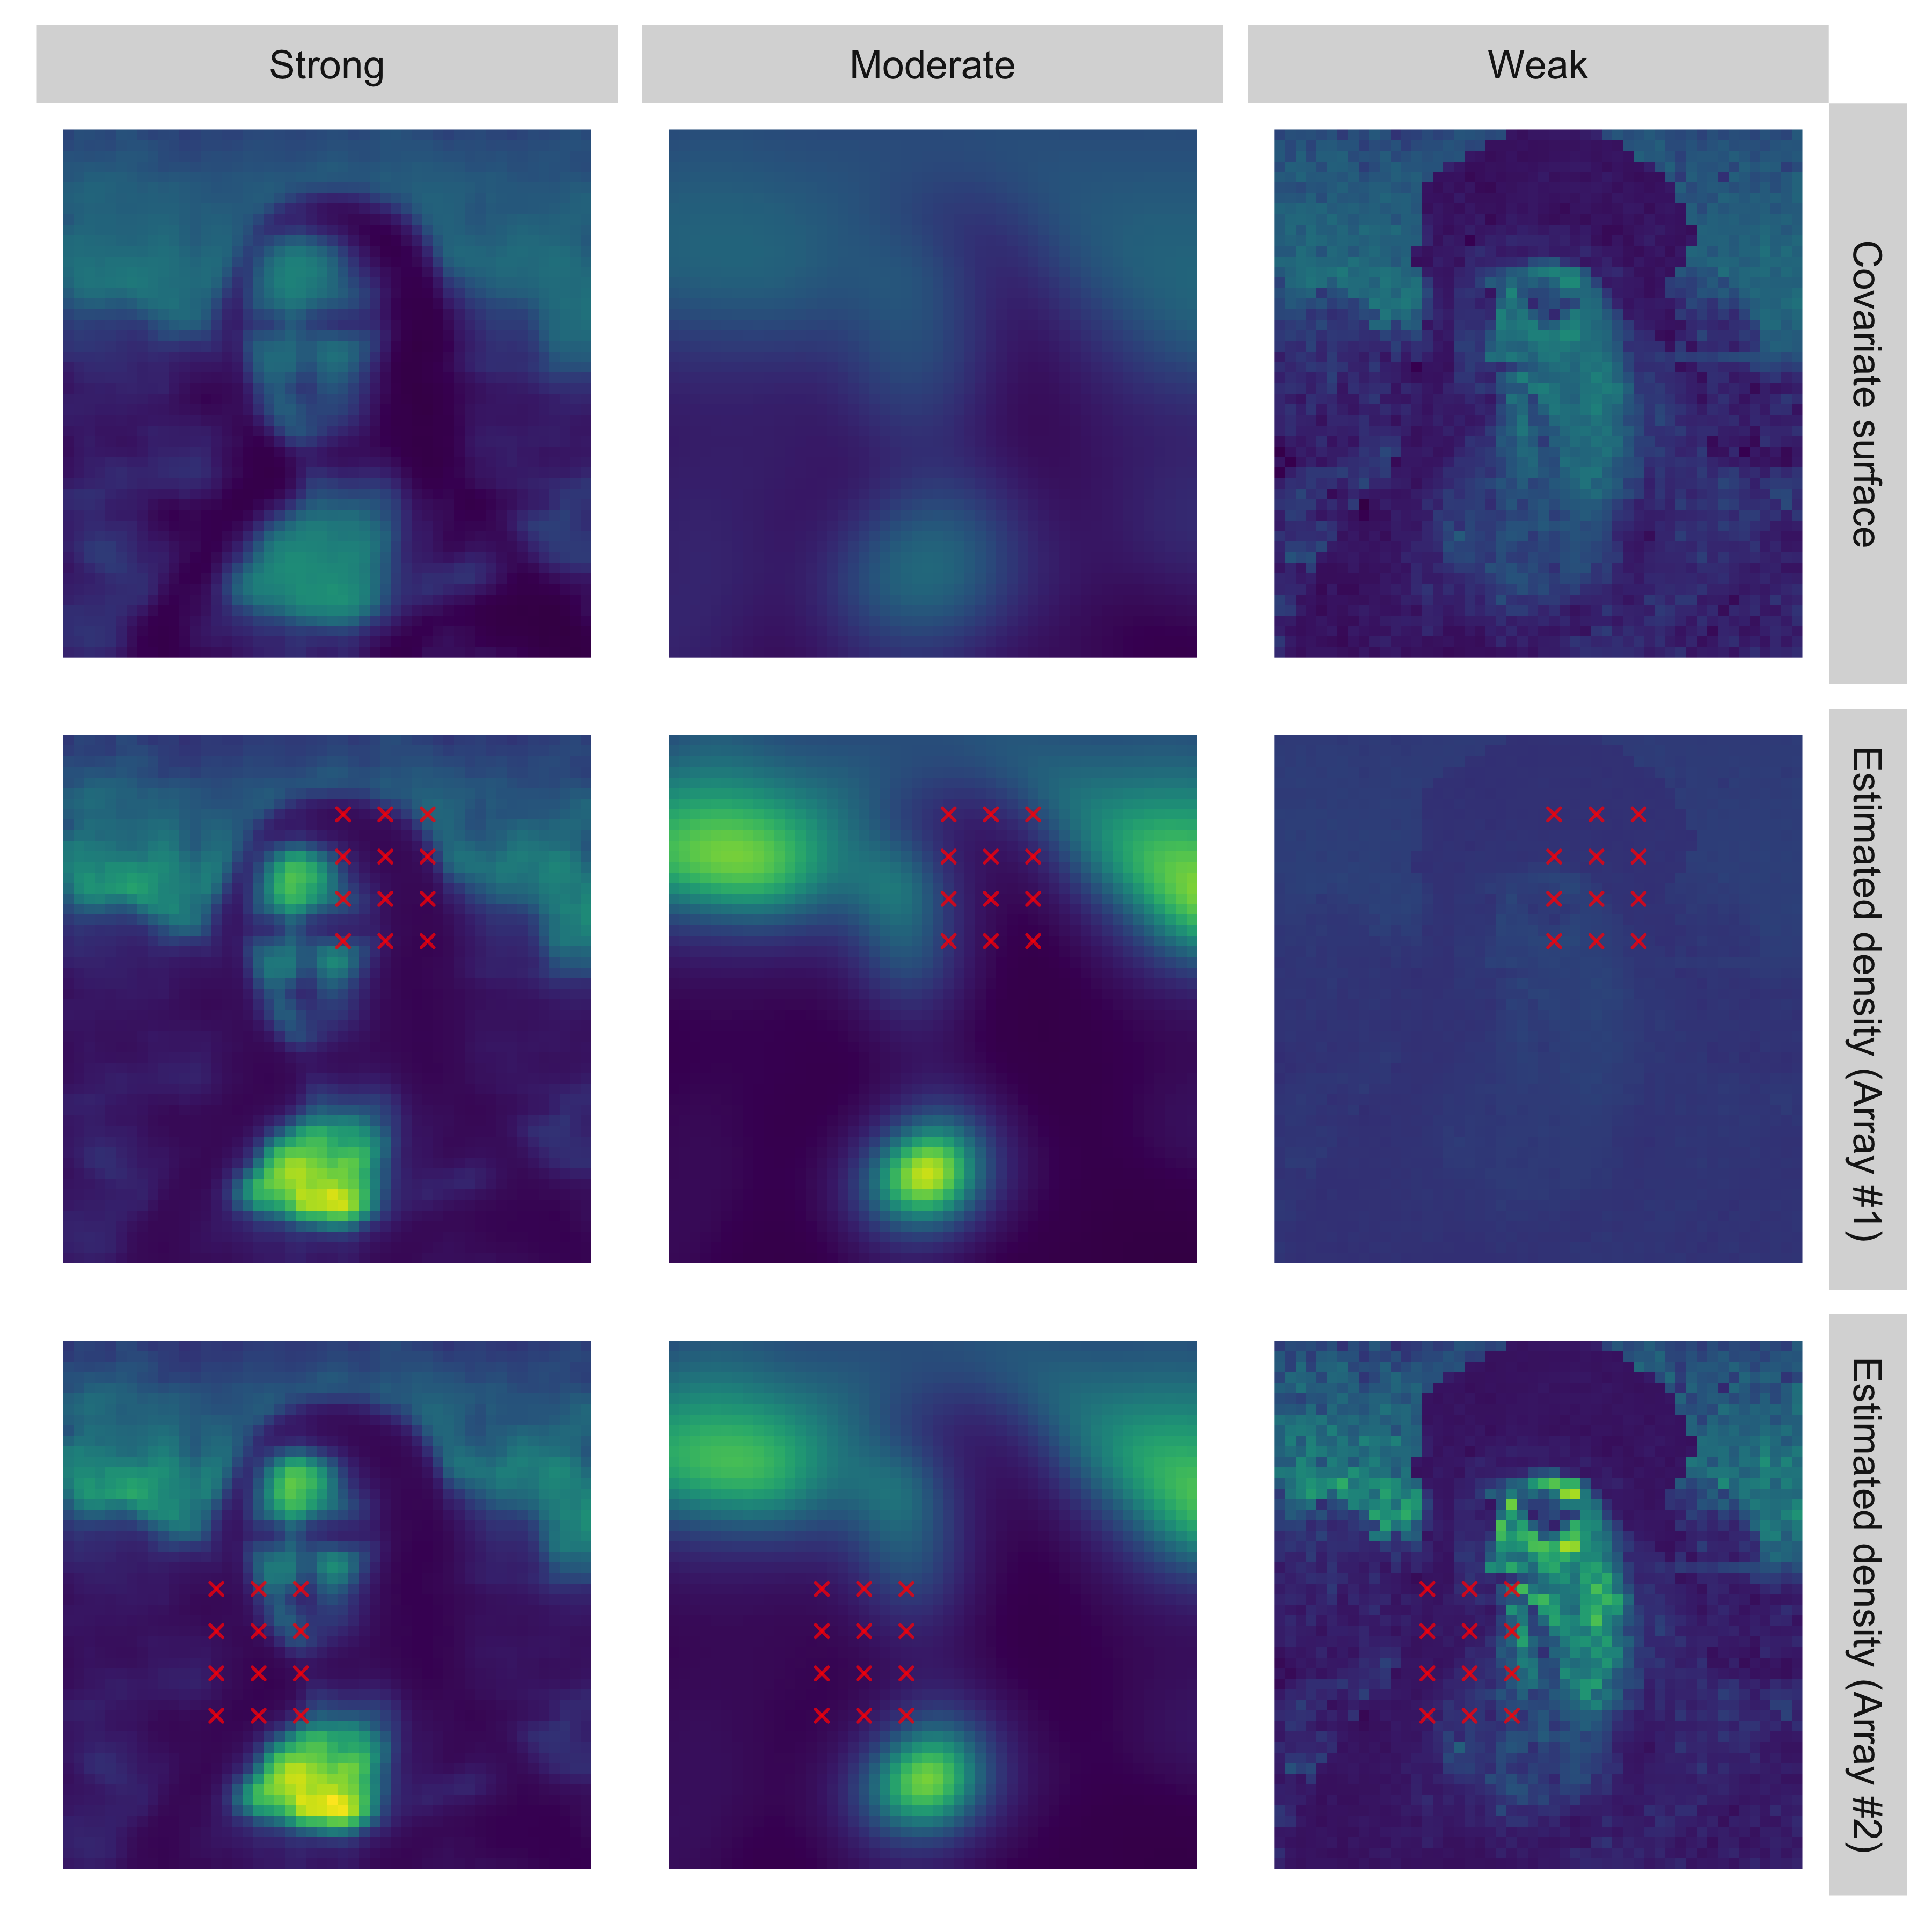
\includegraphics[width=0.8\textwidth]{mona_covariates.png}
\caption{Expected activity center surfaces estimated from a single survey using a model with density a function of one of two simulated spatially-varying covariates. Plot (a) and (d) show the two covariates, obtained by blurring the true density surface in Figure \ref{mlinputs} to a lesser or greater degree, so as to simulate a ``strong'' and ``moderate'' covariate respectively. Plots (b) and (c) show the estimated expected AC surfaces using the covariate surface in (a) and a 4$\times$3 array placed at two different locations, while plots (e) and (f) show similar results for the covariate surface in (d). Plot notation and colour scaling is as for Fig \ref{mona_torch_higheffort}.} 
\label{mona_covariates}
\end{figure}

\subsubsection{AC densities with fewer activity centers}


\begin{figure}[htbp]
\centering
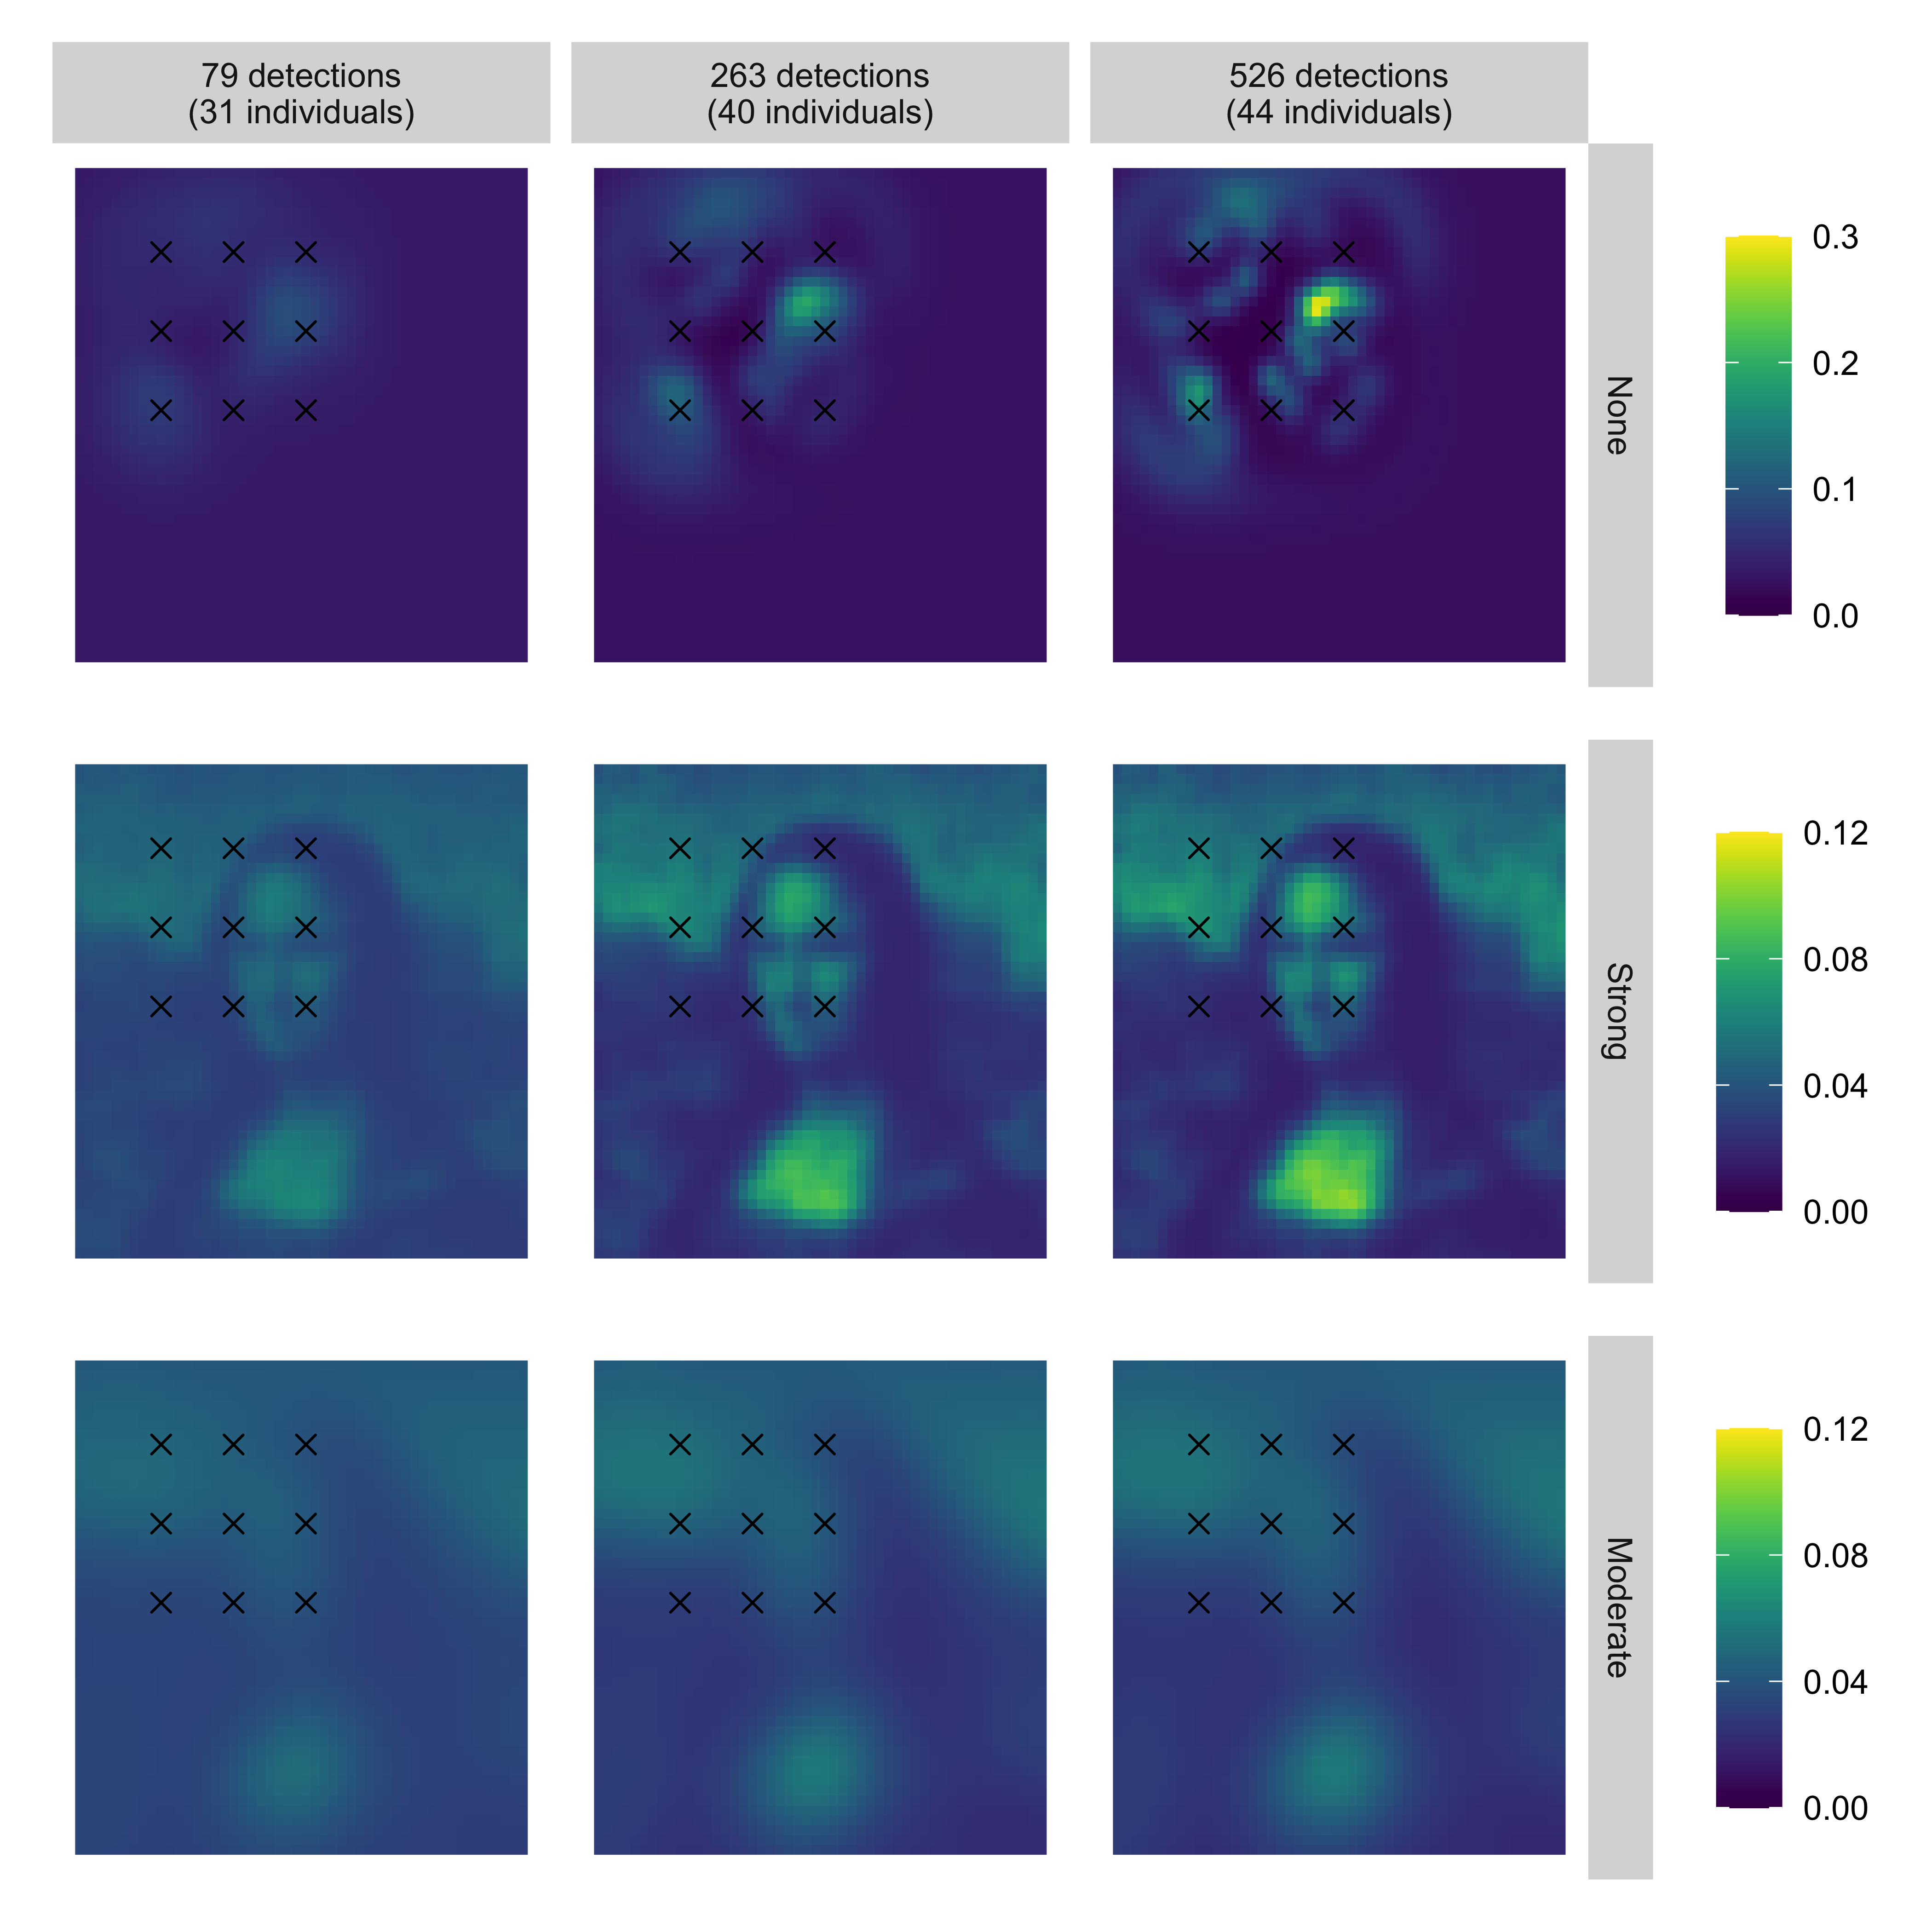
\includegraphics[width=1\textwidth]{mona_peaky_avgd.png}
\caption{Estimates of realised AC density surfaces from a constant density model (first row) and expected activity center density surfaces from a model with density depending on ``Strong'' or ``Moderate'' covariates (second and third rows respectively). The 84 realised activity centers are shown in the ``Realisation 2'' plot of Figure~\ref{mlinputs}. Detectors are shown as crosses. Results are averaged over 100 simulated surveys.}
\label{mona_peaky_avgd}
\end{figure}

Figure~\ref{mona_peaky_avgd} shows the average realised AC density (top row) and the expected AC density (middle and bottom rows) for smaller sample sizes  from 100 simulations. An average of 31, 40 and 44 of the 84 ACs present in ``Realisation 2'' of Figure~\ref{mlinputs} was detected, giving average numbers of detections of each detected individual of 2.5, 6.6 and 12, respectively.

Notice that the estimates of the realised AC surface (top row) (a) do not really recover the Mona Lisa in any recognisable way, (b) become more ``spiked'' (density concentrated more closely around ACs) inside the array as sample size increases, and (c) predict flat density far from the array. We discuss each of these features below.

Regarding (a), realised AC surfaces are not designed to recover the expected density (which is what the Mona Lisa image is), they are designed to estimate the location of ACs and reflect the uncertainty in this estimation. Point (b) is a consequence of this: as sample size increases, the amount of information on where the ACs in the vicinity of the detectors are increases and hence the probability density of AC location contracts about the AC locations. Point (c) is another consequence: because ACs far from the array are not detected, there is no information in the sample on their location other than that contained in the SCR estimate of mean density, and so all the model ``knows'' about AC location far from the array is that they occur in space at the estimated mean density of ACs. 

We also note that because Figure~\ref{mona_peaky_avgd} shows estimates averaged over 100 simulations, the realised AC densities in the plot are smoother than would be obtained from any single survey. An example from a single survey is shown in Figure \ref{move}.

%We observed similar patterns under the more ``wildlife survey appropriate'' condition in which we generated only 85 activity centers across the study region (Figure \ref{peaky}). In this case there is a large difference between the mean intensity surface (the Mona Lisa) and the activity center surface in this realization (85 points), and so it is not surprising that the estimated realised AC density surface looks nothing like the Mona Lisa (Figure \ref{peaky}, first row). Nevertheless, a model assuming constant density gives increasingly accurate estimates of the locations of activity centers in the vicinity of detectors as survey effort increases, but very little information is obtained elsewhere, and this does not change with survey effort (Figure \ref{peaky}, first row). This gives the estimated activity center surfaces a characteristic pattern -- the surface becomes increasingly peaked or ``spiky'' around detectors as survey effort increases, but remains flat away from the array. 

%Any covariate model returns a surface that is some multiple of the covariate surface. Whether this is a good approximation of the true mean intensity surface depends on the strength of the covariate and sample size. With a strong covariate and sufficient sampling occasions we recovered the Mona Lisa, but with only a single occasion the direction of the relationship was incorrectly estimated, so that dark areas were predicted as light and light areas as dark (Figure \ref{peaky}, second row). This error was corrected by additional occasions. The same pattern occured with a moderate covariate, but the effect of the weaker covariate is clear in that we did not recover as good an approximation of the Mona Lisa (Figure \ref{peaky}, third row). Additional sampling would not help with this. Note that in both cases the surface we recovered is an approximation of the mean intensity surface. It does not give a good approximation to the locations of the 85 activity centers in this particular realization.

Estimates of the expected AC density surface recover the Mona Lisa image well in the ``Strong'' covariate relationship scenarios (middle row of Figure~\ref{mona_peaky_avgd}), with greater focus as sample size increases and hence the amount of information about the relationship increases. The same is true in the case of the ``Moderate'' covariate scenarios (bottom row), but with a weaker relationship between covariate and true density, the image is more blurred, i.e. the covariate cannot pick out the high-resolution features of the density surface.

\subsubsection{Realised usage densities with few activity centers}

Estimates of realised usage density surface estimates are shown in Figure~\ref{move}. The realised usage surfaces add an encounter function that is fairly insensitive to sample size, around the realised AC surface (see Appendix~\ref{appx:usage-details} for details). This dilutes the effect of the realised AC surface concentrating around ACs as sample size increases and results in a smoother surface. Realised usage surfaces are higher than realised AC surfaces because each single AC generates multiple points of usage.

%The  realised usage density surfaces are not just smoothed versions of the realised AC surfaces, however. In our example unobserved animals were estimated to be spending their time on the outskirts of the study region, far away from any detectors (Figure \ref{move}, second row), which is quite different from the homogenous surface when considering only at activity centers (Figure \ref{move}, first row). In contrast, the realised animal density surface for captured animals {\it was} essentially a smoothed version of the realised activity center surface around the detector array, and so very similar in terms of the broad patterns it showed (Figure \ref{move}, third row).

\begin{figure}[htbp]
\centering
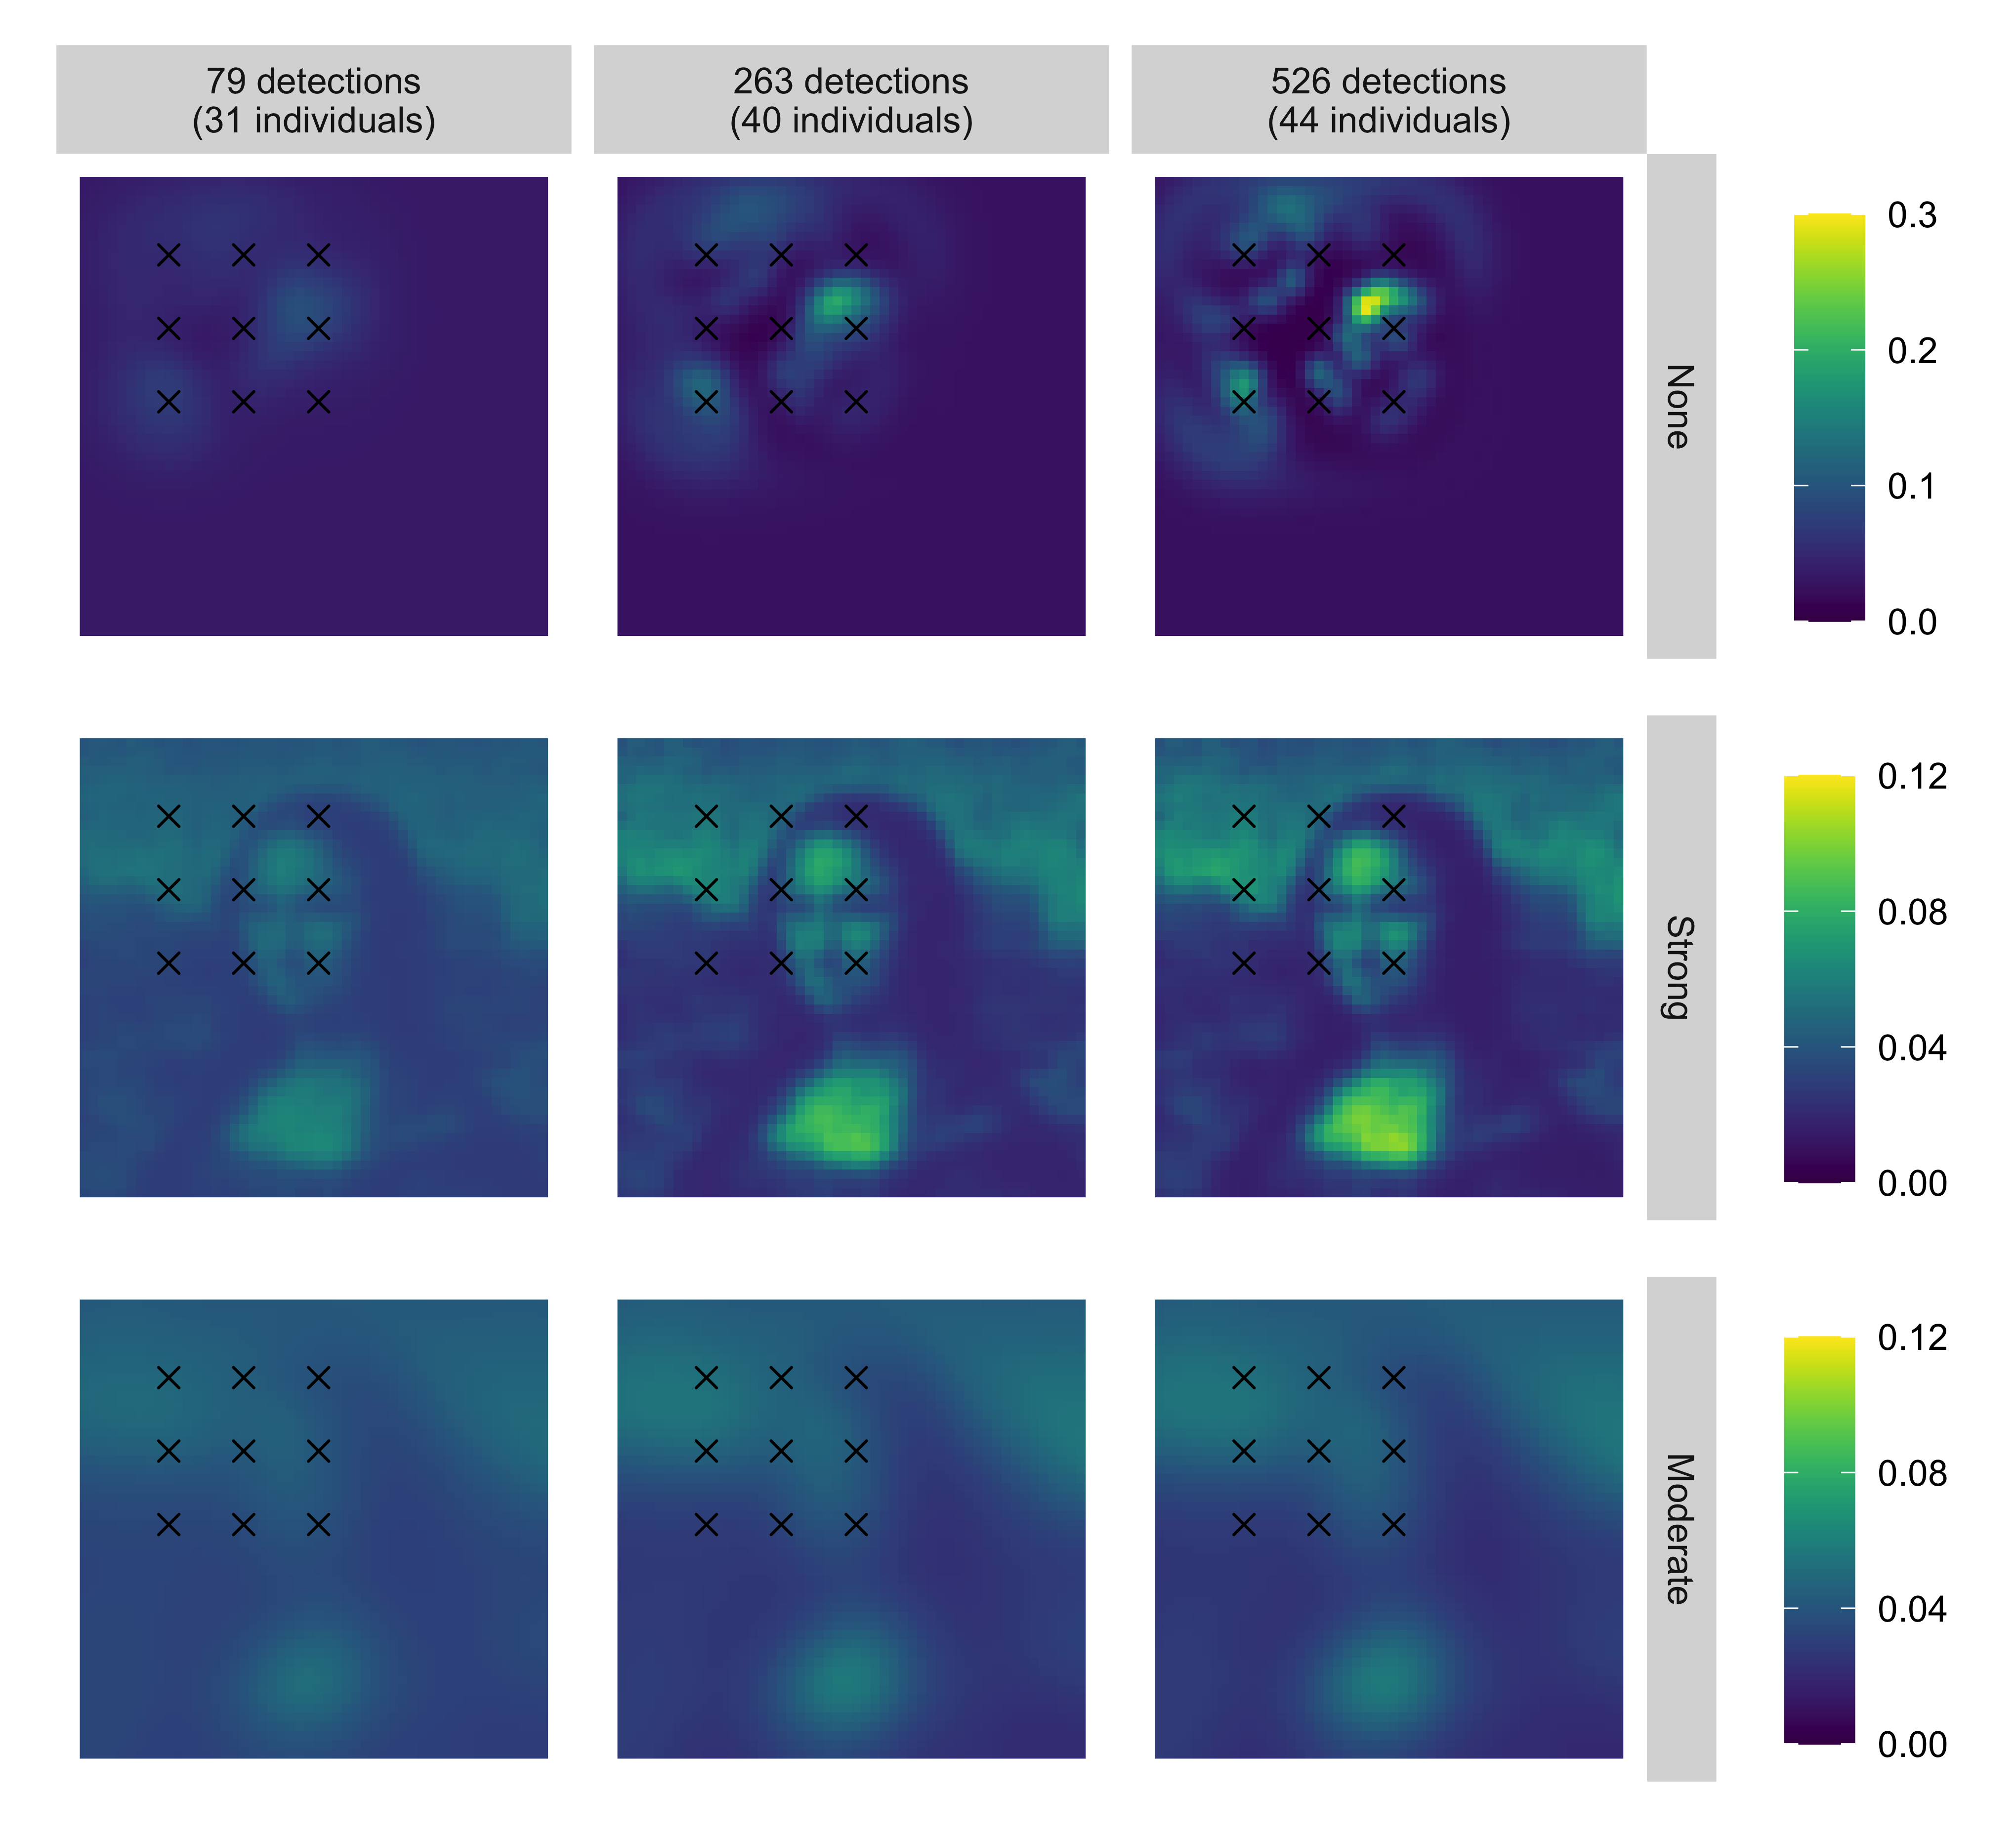
\includegraphics[width=1\textwidth]{mona_with_movement.png}
\caption{Estimates of realised AC density surfaces from a constant density model (first row) and the corresponding realised usage surfaces (second row, note that colour is shown on a log scale), for both observed and unobserved animals. Detectors are shown as crosses. Results are from a single simulated survey.}
\label{move}
\end{figure}

\section{Camera-trap survey of tigers in Nagarahole, India}

\subsection{Materials and methods}
We reanalysed data obtained from a camera trap survey of tigers {\it Panthera tigris} living in and around the Nagarahole Tiger Reserve of Karnataka, India, as reported in \cite{Dorazio+Karanth:17}. A description of the survey can be found in  \cite{Dorazio+Karanth:17}. It used an array of 162 motion-activated camera traps, these being placed at 2–3 km intervals throughout the area (Figure~\ref{tigernocov}, ``All traps''). 

We fit a model assuming constant density, using three different trap arrays. The first array was the same one used in the original study, and from these data we estimate both the realised AC density and the realised usage density. The second array was a subset of traps that excluded about 70\% of the traps, leaving a large region without traps in the interior of the study region (Figure \ref{tigernocov}, ``Subset \#1''). The third used a subset of traps that excluded eight detectors from each of two interior areas of the survey area in which the original survey showed the realised AC density to be particularly high (Figure \ref{tigernocov}, ``Subset \#2''). 

We also fitted a number of covariate models to the three arrays. We investigated models in which density depended on longitude and latitude, as smooths or linear effects. The model selected by AIC included a linear effect of latitude only, and we report results from this model. 


\subsection{Results} 
%The same broad patterns were visible in our reanalysis of the Nagarahole tiger survey (Figures \ref{tigernocov} to \ref{tigerspaceuse}). 

\subsubsection{Realised activity center densities}

The full array of traps used in the original Nagarahole study clearly showed three areas of high realised AC center density in the interior of the study region, along easting $\approx 625$ and northing $\approx 1,324, 1,330$ or $1,336$ (Figure \ref{tigernocov}, ``All traps, no cov.''). 

When we refitted using a subset of traps that excludes traps in the interior of the study region, high realised AC density areas in the interior of the region were replaced by a flat surface indicating a homogenous low density, and the three high density regions described above were not detected  (Figure \ref{tigernocov}, ``Subset \#1, no cov.''). We also observed some regions where estimated density {\it increased} after the removal of the interior traps (see the easternmost detectors in Figure \ref{tigernocov}, ``Subset \#1, no cov.''). %This occurs when animals have their activity centers near to, but outside, the area circumscribed by an array -- estimated activity centers then tend to be pulled towards the traps that they are closest to. 

With the second subset of traps, which exclude eight detectors from each of two high density interior areas, the constant density model still recognized that activity centers are located in these areas, but the estimated locations of these activity centers showed a clear shift from what was found in the original survey (Figure \ref{tigernocov}, ``Subset \#2, no cov.''). The estimated location of the northernmost of the two activity centers moved to the south east, while the other activity center moved to the south.

% ID -- added two options for relative differences v1 and v2. v2 makes change relative to density with all traps if change is negative, and relative to density with reduced set of traps if positive. This makes all changes lie between -100 and +100, and avoids very large positive relative changes where density was tiny in the all traps density surface. Bit weird so I prefer v1, but that makes the colour scales asymmetric (see plot legend). Can squash the blue side but needs more ggplot than I know.
\begin{figure}[htbp]
\centering
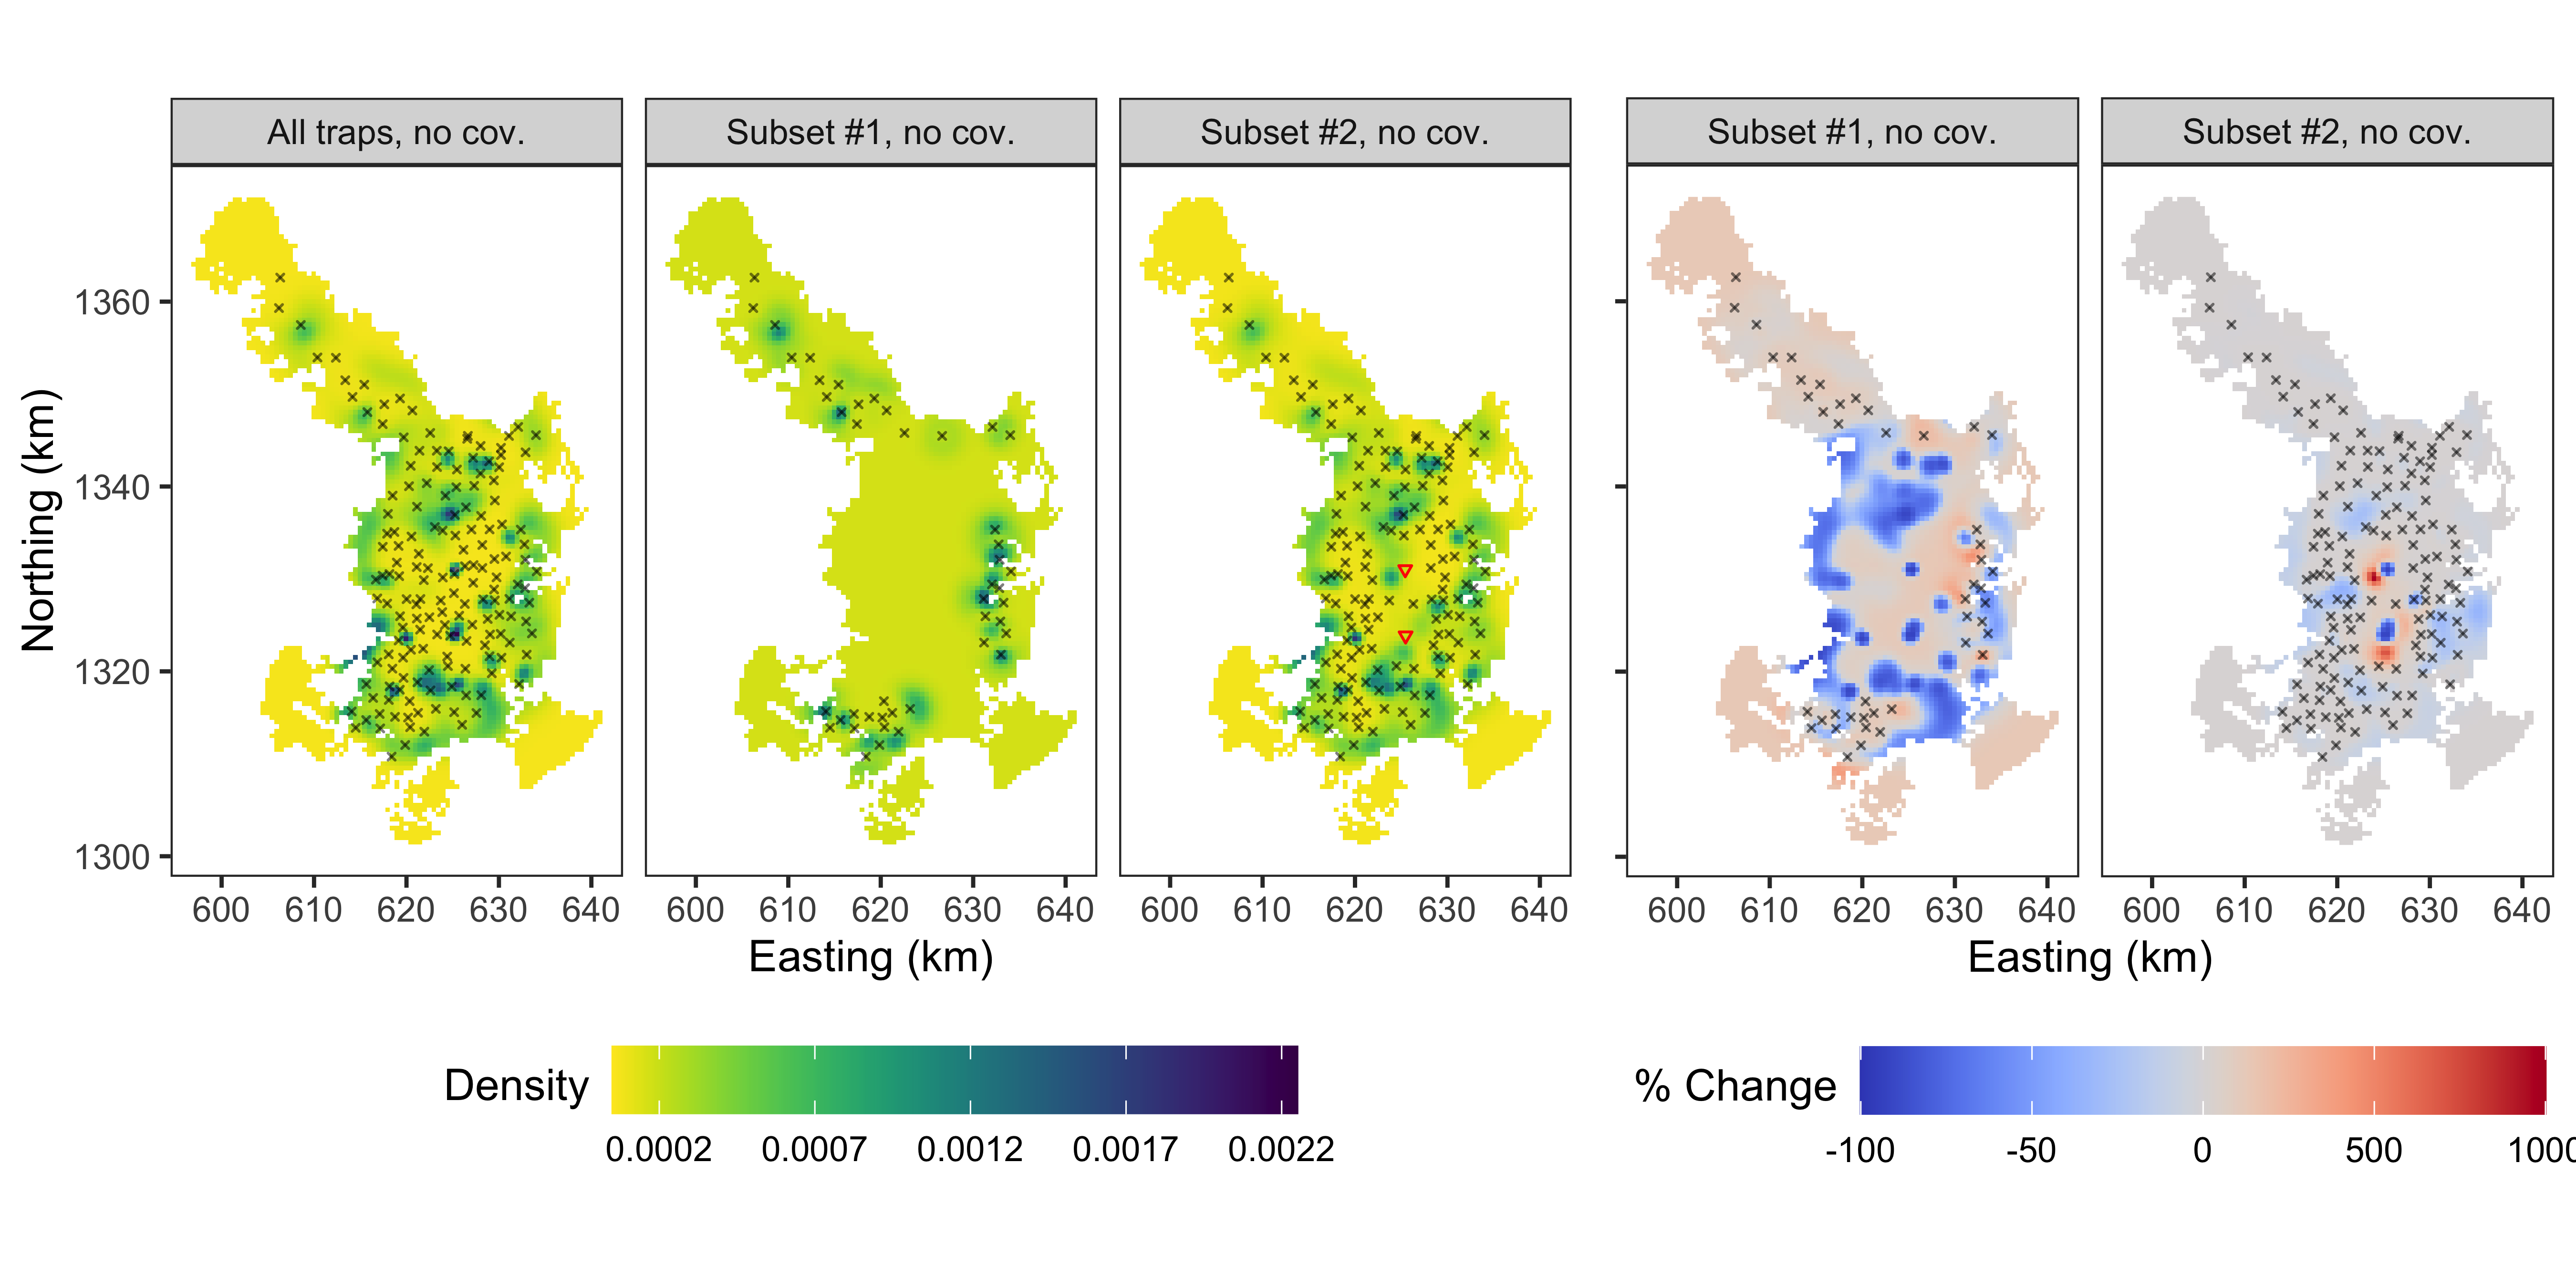
\includegraphics[width=1\textwidth]{tiger_surfaces_nocovs_v1.png}
\caption{Estimated realised activity center densities of tigers in Nagarahole Tiger Sanctuary, India, obtained using different camera trap arrays. Plots (a), (b), and (c) show estimated densities; plots (d) and (e) show differences between the estimated densities obtained using using trap subset \#1 and \#2 and those obtained using all traps. Detectors are shown as black crosses. Red triangles in (c) show the location of what were two high-density spots in (a).}
\label{tigernocov}
\end{figure}

\subsubsection{Expected activity center densities}

The model with the lowest AIC was one in which density depends linearly on latitude. The expected AC density surface obtained from this model showed the estimated density increasing southwards across the region, with density in the extreme south roughly four times that in the extreme north (Figure \ref{tigercov}, ``All traps, northing''). Estimates of expected AC density are much less spatially variable than estimates of realised AC density, and are much less sensitive to changes in the array of traps, providing that the array gives sufficient coverage of the covariate space to estimate the covariate relationship (Figure \ref{tigercov}, ``Subset \#1, northing'' and `Subset \#2, northing''). 

\begin{figure}[htbp]
\centering
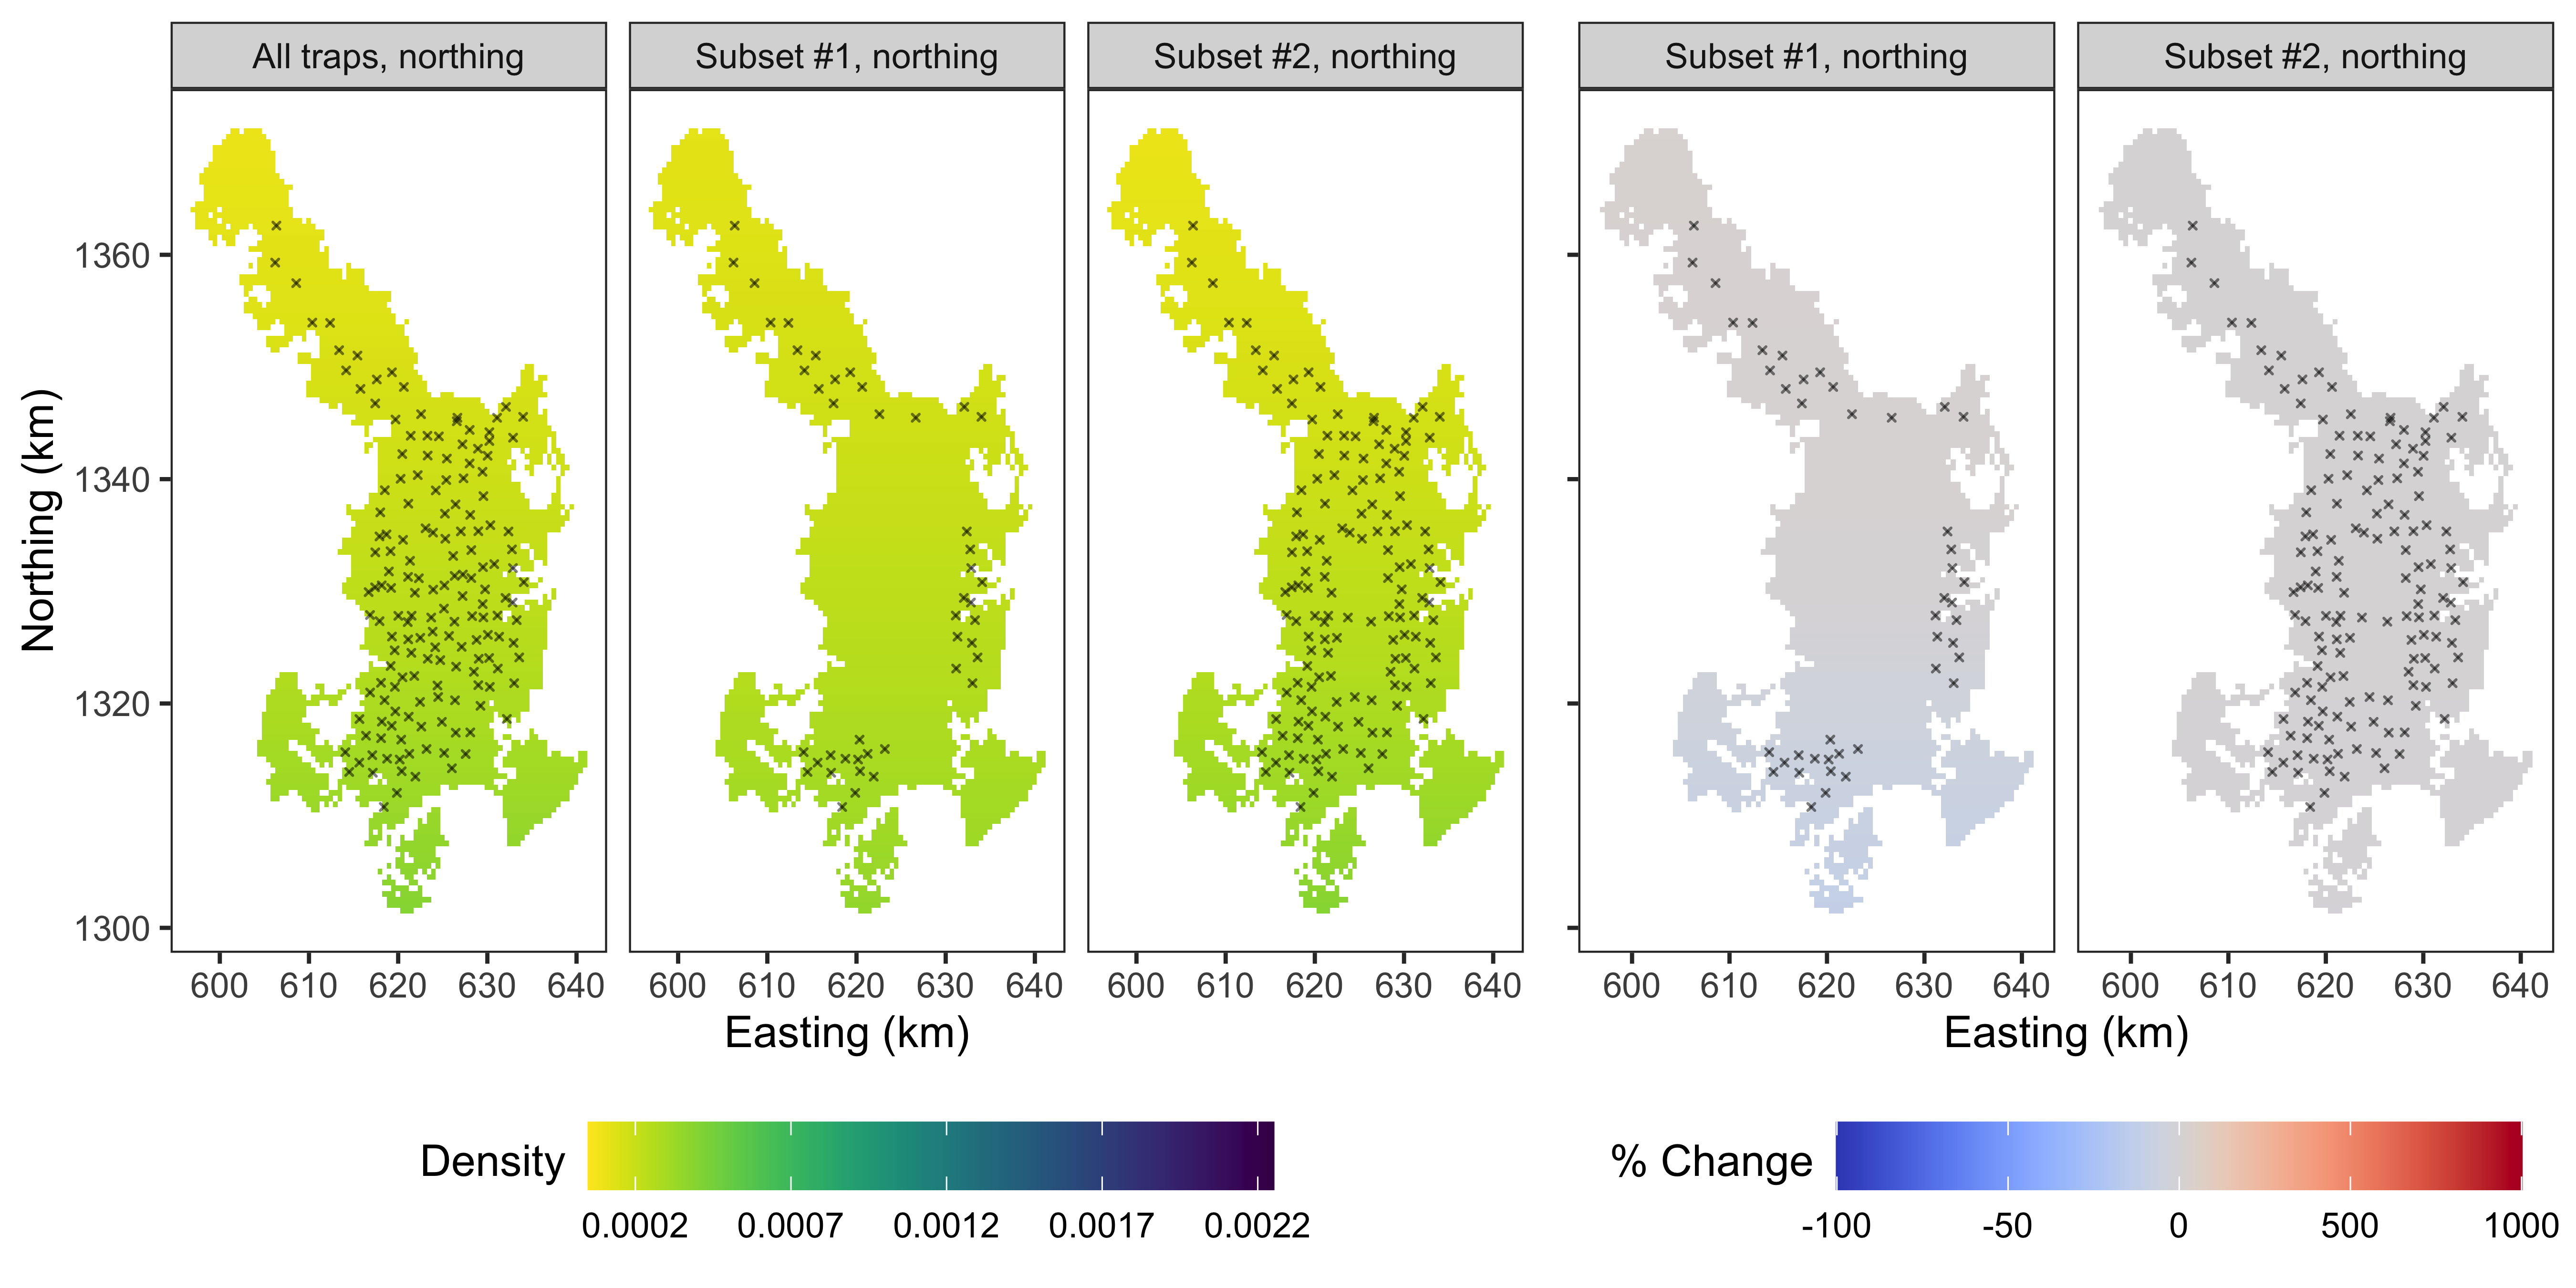
\includegraphics[width=1\textwidth]{tiger_surfaces_covs.png}
\caption{Estimated expected AC density of tigers in Nagarahole Tiger Sanctuary, India, obtained using different camera trap arrays. Plots (a), (b), and (c) show estimates of expected AC densities; plots (d) and (e) show differences between these when using using using trap subset \#1 and \#2, and those obtained using all traps. Detectors are shown as black crosses. The colour scale for (d) and (e) is the same as that for plots (d) and (e) of Figure~\ref{tigernocov}.}
\label{tigercov}
\end{figure}

\subsubsection{Realised usage densities}

An estimate of the realised usage density surface is shown alongside that of the realised AC density surface  in Figure~\ref{tigerspaceuse}. The realised usage density surface is smoother than the realised AC density surface, as expected - because animals ``spread'' themselves about their ACs by moving within their home ranges. % Activity center densities were highest in those cells where sufficient information had been gathered to precisely identify where a single tiger's activity center was. Adding movement to the surface had the effect of dispersing each area of high (activity center) density across a much wider area, the extent of which depended on the estimated range of movement. The estimated spatial scale parameter for the fitted half-normal detection function we used was $\sigma=1.85$km, so that animals can move a substantial distance from their activity centers, relative to the size of the study area. As a result, animal density was highest in areas in which there were several activity centers in relatively close proximity to one another, even if the location of these activity centers was less precisely known than other activity centers. This occured in areas near the southern and south-western borders of the reserve, as well as in a central location near $N=1340$ (Figure \ref{tigerspaceuse}). In contrast, animal density was low in areas that contained only a single activity center, even if the location of the activity center was precisely known (for example at $N=1330$, $E=624$).

\begin{figure}[htbp]
\centering
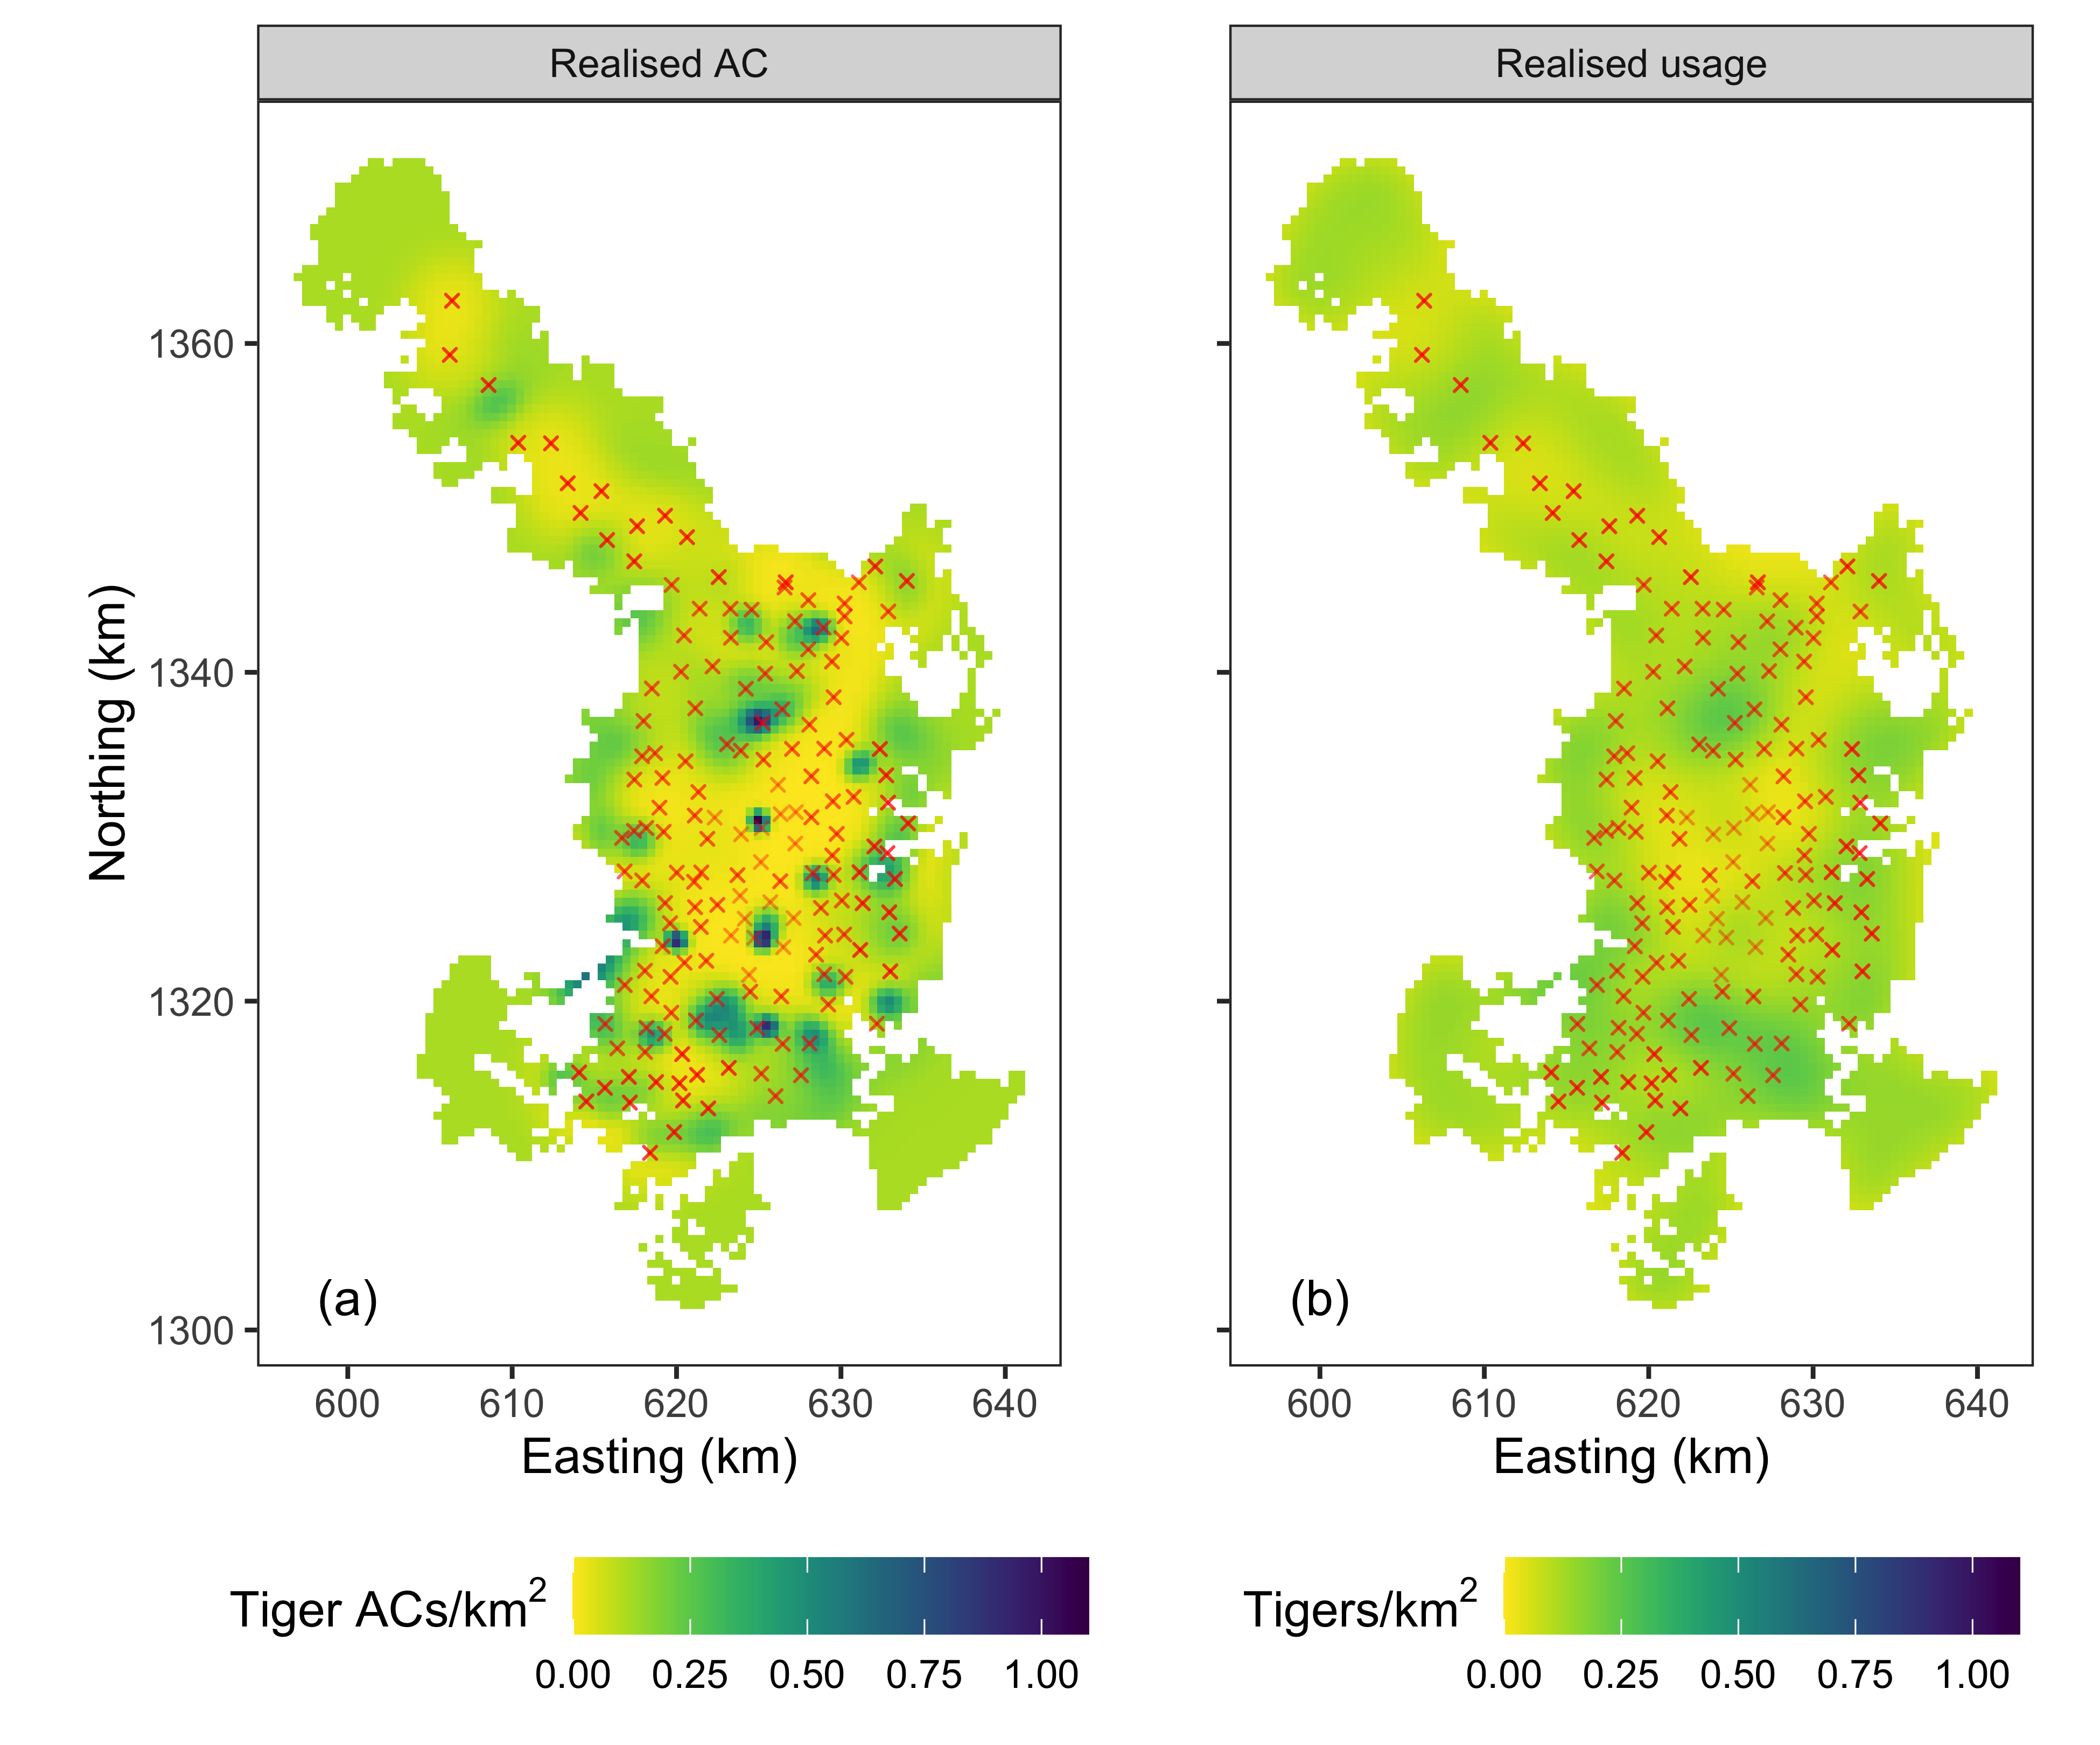
\includegraphics[width=0.6\textwidth]{tiger_spaceuse.png}
\caption{Estimated (a) realised activity center density surfaces from a constant density model and (b) realised animal density surfaces for tigers in Nagarahole Tiger Sanctuary, India. Note that the colour scales for the two plots are different. High density areas are indicated in blue, low density areas in yellow. Detectors are shown as red crosses.}
\label{tigerspaceuse}
\end{figure}


\section{Discussion} \label{discussion}
The realised AC density obtained from an SCR model cannot be interpreted as a species distribution model. Species distribution models predict where species are likely to occur by correlating environmental covariates with species occurrence or species density. %Their rationale is to find favourable habitats and predict that animals will be found in similar habitats across the study region. 
A species distribution model will tend to place higher densities at locations where environmental covariates are most favourable for the species, and spatial variation in the density surface will depend on how environmental covariates change across space and the strength of the relationship between the covariates and species density.

In contrast, high realised AC density occurs where the model is most certain that an activity center is located. Crucially, location of high- and low-density regions of a realised AC density surface depends on (a) where detectors are located (if one was using SCR to identify areas of high density e.g.\ for conservation purposes, or to locate animals, different areas would be identified depending on where the array was placed), and (b) on survey effort (with higher effort resulting in higher troughs and spikes in the realised AC density surface. Different arrays produce quite different estimates for exactly the same AC locations. A useful metaphor here is of SCR as a torch shining a light onto the true activity centers -- what you see depends on where you shine the torch (detector locations) and how brightly you shine it (survey effort). If you interpret the uniform darkness outside of the beam to mean that everything outside the beam is the same, you fundamentally misunderstand the nature of torches and will draw fundamentally incorrect conclusions.

Realised AC surfaces tend to be flat away from where detectors are located. It is important to understand that this flatness reflects a lack of knowledge about the density surface away from detectors, and does not mean that the density surface is flat away from detectors. This point is clearly stated in \cite{{Royle+al:13a}}\footnote{They say: ``As we move away from `where the data live' (away from the detector array) we see that the density approaches the mean density. This is a property of the estimator as long as the detection function decreases sufficiently rapidly as a function of distance. ... predictions tend toward the global mean as the influence of data diminishes'' \citep[p165-166][]{Royle+al:13a}} but is misinterpreted whenever researchers explicitly or implicitly treat realised activity center densities as maps of the spatial distribution of activity centers across the study area. %An exception is when the study region is fully covered by a dense array of detectors, effectively shining an SCR ``torch'' on the whole region. 

Another way to see that flatness away from detectors reflects uncertainty rather than homogenous density is to plot lower and upper percentiles at each pixel, rather than just the posterior mean -- the differences between these percentiles would be large away from detectors and small close to detectors. It seems that this is rarely done, or at least reported in the literature; a practice that would be worth changing. 

%More importantly for people actually conducting SCR surveys is that the realised density estimates obtained close to detectors (and even inside the detector array) {\it also} depend on where detectors are located. The inset plots of Figure \ref{mona1low} and \ref{mona1hi} show the same region in space, and this region lies within a $2.5\sigma$ range of all detector arrays, where one would expect to be making inferences about activity centers. We obtained very different density surfaces in this area depending on where detectors were located. 

When considering realised ACs, SCR models answer the question ``where is an animal with {\it this} spatial capture history likely to have its activity center?'' The answer is always contingent on where detectors are located - because the capture history depends on where the detectors are located. %Changing the locations of detectors also changes the expected capture history, and thus the answer to the question of where the activity center is located. 
This is the case regardless of whether one works in a Bayesian or frequentist framework. The same is true of the realised AC density surface, which simply sums estimated activity centers across animals. In this case the question being addressed is ``Where are the animals with {\it these spatial capture histories} likely to have {\it their} activity centers?'' The dependency on detector location applies to activity centers estimated for detected animals and for those that were not detected. In the latter case we have limited information and the answer to the question for them is really just ``nowhere near where detectors are located''. 

None of this precludes realised AC density surfaces from being useful sources of information, but they do need to be interpreted with care. For practical purposes this means always interpreting them with the caveat that they depend on where detectors are located. Realised AC densities do not give proper answers to questions like ``where are the high- and low-density regions?'' because the highest and lowest points of the surface will always be at or near detectors; not because these are high- or low-density regions of space, but because this is where the capture histories make us most certain that animals are, or are not, present. They also cannot answer questions like ``are animals clustered in space?'' or ``is animal density heterogeneous?'' because the realised density surface will always exhibit variability, even if animal densities are truly a realisation of a homogeneous Poisson point process.

%When estimating the location of a given activity center, the bias caused by detector locations is lowest if the activity center occurs near the center of a dense array of detectors, and is highest if detectors are all on one side of the activity center or if detections are only made at a single detector. Thus bias can be reduced by using a design that makes it likely that all activity centers in the study region are surrounded by a network of detectors. This will be unachievable for most wildlife surveys, as it requires a large number of detectors covering an area beyond the study region, and ideally placed at random {\it [[[note: I say `beyond the region' so that activity centers at the borders are also in the center of some array, but not sure this is correct -- ????]]]} . In summary, it is incorrect to interpret the realised activity center density surface as if it indicated where animals currently have their activity centers. \todo[inline]{DLB: The paragraph above seems both redundant (we have already made the point about misinterpretation of activity density surfaces quite well I think), and unclear in that I don't know what ``bias'' is being referred to in it. I suggest we remove the paragraph.}

There is a way of using SCR so that it can be interpreted as a species distribution model -- by modelling the mean intensity of the underlying process as a function of environmental covariates. Covariates allow one to see beyond the spatial extent of the array (see Figure~\ref{mona_peaky_avgd}), provided that the relationship between covariate and response is a good one, and that detectors cover a sufficient range of covariate values to estimate that relationship well. The resulting surfaces are no longer strongly tied to one particular realisation of the Poisson process. Rather, they show the (estimated) intensity of the underlying process assumed to generate activity centers. These expected densities will be highest where environmental covariates are most favourable (such as further south in Figure \ref{tigercov}). They  answer the questions ``Where are the high- and low-density regions?'' and ``What spatial variables are good predictors of the high- and low-density regions?'' in a way that is consistent with how this question is answered by species distribution models. %They predict where we would expect to see activity centers, if we were able to observe multiple independent populations distribute themselves across the study region. 

Using covariate models, and associated model-based inference, is not without issues -- there is a danger of extrapolating the density surface beyond the range of covariates around the detectors, and the relationship with density and covariate is assumed to be the same everywhere as it is around the detectors. The extent to which the expected activity center surface predicts where animals have their activity centers {\it in this realization of the process} depends on the strength of the covariate relationship and on the number of activity centers, each of which is assumed to be an independent draw from the underlying process. %In the Nagarahole survey, for example, there is a relatively weak northing covariate and a relatively small number of activity centers, and the estimated expected activity center density surface provides very little information about the location of current activity centers. 

The concept of an activity center is central to SCR models, but for many applications of SCR it may be more appropriate to consider a distribution of space use, taking into account all locations where an animal may have been present, rather than a distribution over activity center locations only. The detection function or encounter function estimated as part of an SCR model provides information about how far from its activity center an animal may move. This can be easily integrated with the estimated realised AC density to give an estimated realised {\it usage} density surface. The resulting surface effectively smooths the realised AC density surface, with the amount of smoothing determined by the distances that animals move. As it is based on realised AC density, the usage density surface also depends on where detectors are located and on survey effort. However, it depends less heavily on these factors than the realised AC surface because the detection function or encounter function does not depend on them. In particular, the realised usage density surface quickly stops becoming increasingly ``peaked'' as survey effort increases.

Ultimately, the appropriate density surface to use depends on the aims of the researcher. We have argued that the estimated realised activity center density surface should not be used as a species distribution model, because of the strong dependence on detector location and survey effort. But if the goal is to identify the activity centers of {\it some} animals currently in the study region (and it does not matter which ones) then it may well be an efficient way of locating these, particularly at the center of the array. If the goal is to actually {\it find} an animal in the study region, then it is less important where animals have their activity centers and more important to know where they spend their time, and the realised usage density surface is most useful. If the goal is to estimate where animals (not just the ones in the current realisation) are likely to have activity centers, then this is a species distribution question and the expected AC surface, with density a function of covariates, should be used.

\section{Conclusions}
%This paper demonstrates that the summed posterior distribution of estimated ranges across animals obtained from SCR -- what we call the realised activity center density surface -- cannot be used as a species distribution model. We illustrated this point in a number of ways, first with a binomial point process, then by using the Mona Lisa to simulate a Poisson point process, and finally using data from a real-world camera detector survey. All these examples returned the consistent message that realised activity center density surfaces differ depending on detector location. This dependency is most obvious at large spatial scales, where moving a detector array is like ``shining a torch'' on a particular part of the study area, but is also present within the region in and around the detector array itself. 

Our main messages are:
\begin{enumerate}
\item Realised activity center density surfaces cannot be interpreted as SDMs. This is both because these surfaces draw inferences about one realisation of a spatial point process, whereas SDMs make inferences about the long run average of the process; and because the surface depends systematically on where detectors are located.
\item The realised activity center density surface typically shows highest peaks and deepest troughs close to the center of arrays, defaulting to close to the mean of the underlying process away from the array. A flat density away from detectors reflects a lack of knowledge, and not constant density. We should expect that in reality some areas away from detectors have substantial deviations from the process mean -- it is just that we do not know which areas.

\item An SCR model that models mean activity center density as a function of environmental covariates can be interpreted as a SDM. Here the key difference is that the surface obtained from the covariate model -- what we call an expected activity center surface -- is a statement about the mean intensity of the underlying process, and is independent of array location provided that the environmental covariate space has been sufficiently sampled.

\item Realised activity center densities can be extended into realised usage densities. This is done by using the estimated encounter or detection function to ``spread'' animals about their estimated ACs according to the expected number of encounters of the animal as distance from its AC increases. 
\end{enumerate}

%"OK everyone, put your detectors where you'd like to shine your torch, and you'll get a perfectly good estimate of animal density there using our posterior AC map".

\bibliographystyle{mee}
\bibliography{monalisa}

\clearpage
\appendix
\appendixpage
\section{Realised AC and usage density surfaces}
\label{appx:usage-details}

This appendix defines the realised activity centre (AC) surface and the realised usage surface. Let $\bm{x}$ be an AC location (a point in the survey region, which has surface area $A$), $\bm{\omega}$ be a spatial capture history, and $f(\bm{x})$ be the probability density function (PDF) of $\bm{x}$ ($f(\bm{x})=1/A$ when density is uniform in the survey region). The PDF of $\bm{x}$, given $\bm{\omega}$ for a single animal is then
\begin{eqnarray*}
f(\bm{x}|\bm{\omega})&=&\frac{P(\bm{\omega}|\bm{x})f(\bm{x})}{\int P(\bm{\omega}|\bm{x})f(\bm{x})\;d\bm{x}}.
\end{eqnarray*}
\noindent
where integration is over the whole survey region.

The realised AC density when there are $N$ animals in the region, of which $n$ are detected and the $i$th detected animal has capture history $\bm{\omega}_i$ is defined as
\begin{eqnarray*}
f_\cdot(\bm{x}|\bm{\Omega})&=&\sum_{i=1}^nf(\bm{x}|\bm{\omega}_i)\;+\;(N-n)f(\bm{x}|\bm{\omega}_0)
\end{eqnarray*}
\noindent
where $\bm{\Omega}=(\bm{\omega}_1,\ldots,\bm{\omega}_n)$ and $\bm{\omega}_0$ is the zero capture history (not detected at any detector).

Now let $\mu(\bm{u}|\bm{x})$ at a point $\bm{u}$ in the plane be an animal's expected usage intensity at the point, given that an animal has its AC at the point $\bm{x}$.
%suppose that there is a point process with intensity $\mu(\bm{u}|\bm{x})$ at a point $\bm{u}$ in the plane, that governs an animal's usage at the point, given that an animal has its AC at the point $\bm{x}$ (the interpretation being that each point of this process defines a point in space that was used by the animal).
We define the realised usage density of the animal at $\bm{u}$, given its capture history $\bm{\omega}$ to be 
\begin{eqnarray*}
u(\bm{u}|\bm{\omega})&=&\int \mu(\bm{u}|\bm{x})f(\bm{x}|\bm{\omega}_i)\;d\bm{x},
\end{eqnarray*}
\noindent
where integration is over the whole survey region.

The realised usage density for the population of $N$ animals is then defined as
\begin{eqnarray*}
u_\cdot(\bm{x}|\bm{\Omega})&=&\sum_{i=1}^nu(\bm{x}|\bm{\omega}_i)\;+\;(N-n)u(\bm{x}|\bm{\omega}_0).
\end{eqnarray*}

To implement this, we discretize the survey region into a mesh of $M$ pixels and set the expected usage function $\mu(\bm{u}_m|\bm{x})$ for pixel $\bm{u}_m$ ($m=1,\ldots,M$) to be equal to the encounter function (the expected number of times an animal with AC at $\bm{x}$ visits the pixel). In our application we used
\begin{eqnarray*}
\mu(\bm{u}_m|\bm{x})&=&\lambda_0\exp\left\{-\frac{\lVert \bm{x}-\bm{u}_m\rVert^2}{2\sigma^2}\right\}.
\end{eqnarray*}


\section{Bayesian Inference}
\label{appx:Bayesinference}

\textbf{\textit{This appendix remains to be created}}.







\end{document}
